\documentclass{ntuthesis}

\usepackage{times}
\usepackage{verbatim}
\usepackage{color}
\usepackage{url}
\usepackage{graphicx}
\usepackage{array}
\usepackage{hhline}
\usepackage{qtree}
%\usepackage{caption}
\usepackage{tikz}
\usepackage{tikz-qtree}
\usepackage{pgfplots}
\usetikzlibrary{shapes,arrows,fit,positioning}
\pgfplotsset{compat=newest}
\usepackage{multicol}
\usepackage{amsmath}

\usepackage{multirow} 
\usepackage{rotating}

\usepackage{algorithm}
%\usepackage{algorithmic}
\usepackage{algpseudocode}

\usepackage{subcaption}

% Format the refs
\usepackage[sort,comma]{natbib}
\usepackage[hidelinks]{hyperref}

\usepackage{titlesec}
\usepackage{titletoc}
\usepackage{etoolbox}

% Centering the ToC's title
\usepackage{tocloft}

% Include ToC/LoF/LoT into ToC
\usepackage[notbib]{tocbibind}

% Include outside .pdf
\usepackage{pdfpages}

% Add wallpaper
\usepackage{wallpaper}

% 2 words indent in first line for Chinese
\usepackage{indentfirst}
\setlength{\parindent}{2em}

\usepackage{etoolbox}
\newrobustcmd{\disambiguate}[3]{#2,~#3}

\usepackage{mathtools}
\newcommand\undermat[2]{%
\makebox[0pt][l]{$\smash{\underbrace{\phantom{%
\begin{matrix}#2\end{matrix}}}_{\text{$#1$}}}$}#2}

\newcommand\underscope[2]{%
\makebox[0pt][l]{$\smash{\underbracket{\phantom{%
\begin{matrix}#2\end{matrix}}}_{\text{$#1$}}}$}#2}

\newcommand\overscope[2]{%
\makebox[0pt][l]{$\smash{\overbracket{\phantom{%
\begin{matrix}#2\end{matrix}}}^{\text{$#1$}}}$}#2}

% Using the tex-text mapping for ligatures etc.
\defaultfontfeatures{Mapping=tex-text}

% Set the default fonts
\setmainfont{Times New Roman}
%\setCJKmainfont{楷體-繁}
\setCJKmainfont{標楷體}
% value > 0
\def\xeCJKembold{0.4}

% hack into xeCJK, you don't need to understand it
\def\saveCJKnode{\dimen255\lastkern}
\def\restoreCJKnode{\kern-\dimen255\kern\dimen255}

% save old definition of \CJKsymbol and \CJKpunctsymbol for CJK output
\let\CJKoldsymbol\CJKsymbol
\let\CJKoldpunctsymbol\CJKpunctsymbol

% apply pdf literal fake bold
\def\CJKfakeboldsymbol#1{%
  \special{pdf:literal direct 2 Tr \xeCJKembold\space w}%
  \CJKoldsymbol{#1}%
  \saveCJKnode
  \special{pdf:literal direct 0 Tr}%
  \restoreCJKnode}
\def\CJKfakeboldpunctsymbol#1{%
  \special{pdf:literal direct 2 Tr \xeCJKembold\space w}%
  \CJKoldpunctsymbol{#1}%
  \saveCJKnode
  \special{pdf:literal direct 0 Tr}%
  \restoreCJKnode}
\newcommand\CJKfakebold[1]{%
  \let\CJKsymbol\CJKfakeboldsymbol
  \let\CJKpunctsymbol\CJKfakeboldpunctsymbol
  #1%
  \let\CJKsymbol\CJKoldsymbol
  \let\CJKpunctsymbol\CJKoldpunctsymbol}
\newcommand\zhbf[1]{\CJKfakebold{#1}}

% Very Naive Chinese Number
\newcommand\naiveZhNum[1]{
\ifnum #1 = 1 
一 
\else \ifnum #1 = 2
二
\else \ifnum #1 = 3
三
\else \ifnum #1 = 4
四
\else \ifnum #1 = 5
五
\else \ifnum #1 = 6
六
\else \ifnum #1 = 7
七
\else \ifnum #1 = 8
八
\else \ifnum #1 = 9
九
\else
#1
\fi\fi\fi\fi\fi\fi\fi\fi\fi
}

% ToC, LoF, LoT centering settings with package tocloft
\renewcommand{\cftloftitlefont}{\hfill \Huge}
\renewcommand{\cftafterloftitle}{\hfill}
\renewcommand{\cfttoctitlefont}{\hfil \Huge}
\renewcommand{\cftaftertoctitle}{\hfill}
\renewcommand{\cftlottitlefont}{\hfill \Huge}
\renewcommand{\cftafterlottitle}{\hfill}

% \titleformat{\chapter}{\centering\Huge\bfseries}{第\naiveZhNum{\thechapter}章}{1em}{}
\titleformat{\chapter}[hang]{\Huge\bfseries}{\thechapter}{1em}{}
\renewcommand{\cftchapleader}{\cftdotfill{\cftdotsep}} % dots for chapters
\titlecontents{chapter}[0em]{}{\makebox[1.5em][l]{\thecontentslabel}}{}{\cftdotfill{\cftdotsep}\contentspage}

\makeatletter
\patchcmd{\@chapter}{\addtocontents{lot}{\protect\addvspace{10\p@}}}{}{}{}
\patchcmd{\@chapter}{\addtocontents{lof}{\protect\addvspace{10\p@}}}{}{}{}
\makeatother

% Your information goes here
% author: Tz-Huan Huang [http://www.csie.ntu.edu.tw/~tzhuan]

% ----------------------------------------------------------------------------
% "THE CHOCOLATE-WARE LICENSE":
% Tz-Huan Huang wrote this file. As long as you retain this notice you
% can do whatever you want with this stuff. If we meet some day, and you think
% this stuff is worth it, you can buy me a chocolate in return Tz-Huan Huang
% ----------------------------------------------------------------------------

% modify by Yong-Siang Shih (shaform) [http://shaform.com/]

% Syntax: \var{English}{Chinese}
\university{National Taiwan University}{國立臺灣大學}
\collage{College of Electrical Engineering and Computer Science}{電機資訊學院}
\institute{Department of Computer Science and Information Engineering}{資訊工程學系}
\title{Chinese Discourse Connective Detection and Disambiguation, and Its Applications in Discourse Parsing}{中文篇章連接詞偵測與消歧,及其在篇章結構分析之應用}
\author{Yong-Siang Shih}{施詠翔}
\studentid{R02922036}
\advisor{Hsin-Hsi Chen, Ph.D.}{陳信希\ 博士}
\defenseyear{2015}{104}
\defensemonth{July}{7}
\defenseday{31}


% Modify some default titles for Chinese
% \renewcommand{\contentsname}{目錄}
% \renewcommand{\listfigurename}{圖目錄}
% \renewcommand{\listtablename}{表目錄}
% \renewcommand{\tablename}{表}
% \renewcommand{\figurename}{圖}
% \renewcommand{\bibname}{參考文獻}

\floatname{algorithm}{Algorithm}
\renewcommand{\algorithmicrequire}{\textbf{Input:}}
\renewcommand{\algorithmicensure}{\textbf{Output:}}

% sentence
\newcounter{sentcounter}
%\renewcommand{\thesentcounter}{\arabic{sentcounter}}

\newenvironment{sent}[2]{
\noindent
\setlength{\leftskip}{2em}
\refstepcounter{sentcounter}
\label{#1}
(S~\thesentcounter)
}{}
\numberwithin{sentcounter}{chapter}


\begin{document}

% 臺大論文浮水印
\input{watermark.tex}

\frontmatter

\makecover

% 口試委員會審定書  
% 以 \makecertification 產生
%\makecertification
% 或匯入外部.pdf檔
%\phantomsection
%\addcontentsline{toc}{chapter}{口試委員會審定書}
%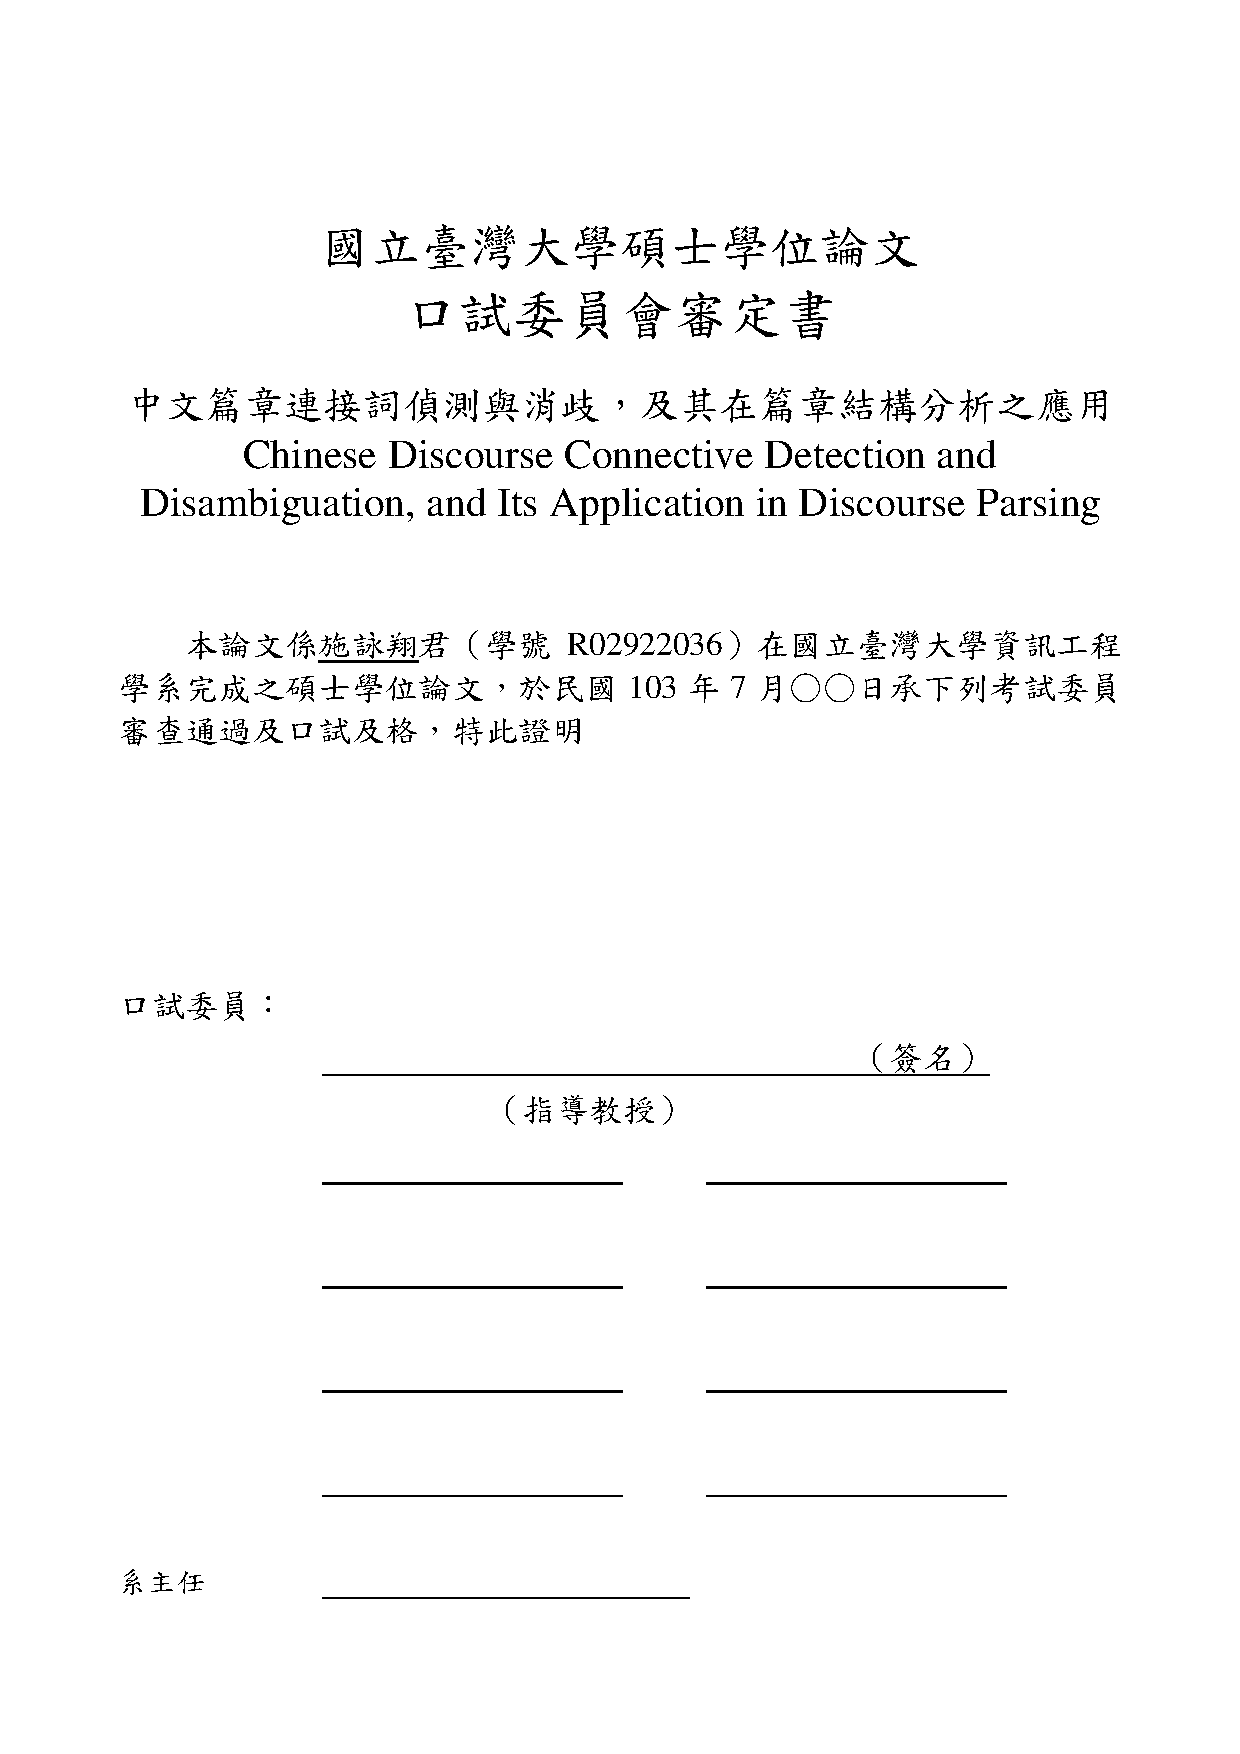
\includepdf[pages={1}]{pdfs/cert.pdf}

% 誌謝
\begin{acknowledgementszh}

在這兩年,首先要感謝我的指導教授陳信希老師的幫助與指導,
讓我能在良好的環境裡順利完成碩論研究。

也要感謝遇到疑問時熱心解答的基鑫學長、瀚萱學長、
昂穎學長、宇錚學長,感謝卿澄學長留下論文模板以及給予許多幫助,
感謝一起努力奮鬥的同學鄧鈞、志杰 、彥賓、 俊杰、衍綺,
感謝幫忙維護工作站的文立以及所有一起學習的同學。

此外也感謝偶爾會在系館遇到的李揚、蔣易、秀萍的加油,
感謝在英辯活動中及校園裡認識的大家的陪伴。

最後則是感謝家人給我的支持。


感謝大家。\\

\hfill 施詠翔\ \ 民國104年7月

\end{acknowledgementszh}


% 摘要
% 中文摘要
\begin{abstractzh}

篇章關係指出了文字單位間如何有邏輯的彼此關聯。
透過分析文章中的篇章結構,我們可以更了解文字的意義。
也因此,篇章結構分析能夠被應用在很多領域,
例如自然語言界面以及大規模的文件分析。

雖然有英文的篇章語料集供研究者使用,中文的大規模語篇資料集一直
到近年才終於被釋出。同時,中文的篇章結構分析有很多獨特的議題,
例如中文的篇章連接詞的種類較多,且常有多個不連續詞語組成的
多重連接詞,此外,中文的句子結構也更為複雜,使得正確辨識篇章結構更為困難。

篇章連接詞是用來辨識中文文章中篇章關係的重要線索,可是由於連接詞
本身的歧義性讓辨識篇章連接詞本身成為一個挑戰。在本篇論文中,
我們研究了跟具有篇章連接詞的顯性篇章關係有關的四個議題:
第一,我們處理篇章連接詞的辨識,在文章中找出可能的篇章連接詞。
第二,我們探討了篇章連接詞的構成詞語間的多重連結關係。第三,我們研究
每個篇章連接詞的篇章關係消歧。最後,我們辨識每個篇章連結詞的論元。

我們提出了不同的特徵來訓練基於羅吉斯迴歸 (Logistic Regression)
演算法的分類器來識別正確的篇章連接詞,以及辨識其篇章關係的種類。
除此之外,我們也排序每個可能的候選連接詞,
並利用一個貪婪的演算法 (greedy algorithm) 來解決連結詞的連結關係歧異性。
最後,我們將論元辨識視為一個序列標記問題 (sequence labeling problem),
並利用條件隨機域 (Conditional Random Fields) 來找出論元的邊界。

除了顯性篇章關係外,隱性篇章關係也需要進一步的研究來加以辨識。
建立在這些元件的基礎上,一個完整的中文篇章結構分析器或能被建造出來。 \\

\noindent
關鍵字:自然語言處理,中文篇章結構分析,篇章連接詞辨識,篇章關係消歧、
論元辨識

\end{abstractzh}

% 英文摘要
\begin{abstracten}

Discourse relations represent how textual units logically connect
with each other. Analyzing the discourse structure for texts
could aid the understanding of the meaning behind the paragraphs.
There are many potential applications such as natural language
interface and large-scale content-analysis.

Although there are popular English discourse corpora for researchers,
large-scale Chinese discourse corpora have not been available until
recently. In addition, Chinese discourse analysis has many
unique issues including the variety of discourse connectives,
the common occurrences of parallel connectives, and the complex
sentence structures.

Discourse connectives are important clues for identifying discourse
relations in Chinese texts. However, the ambiguity involved makes
it a challenge to extract true connectives. In this thesis, we investigate
four tasks regarding explicit discourse relations that are signaled
by discourse connectives. Firstly, we deal with the extraction
of explicit discourse connectives. Secondly, we investigate resolving
linking ambiguities among connective components.
Thirdly, we disambiguate the discourse relation type for each connective.
Finally, we extract the arguments for each discourse connective.

Several features are proposed to train Logistic Regression classifiers
to disambiguate between discourse and non-discourse usages and
the relation types for connectives. Additionally, we rank each
connective candidate and develop a greedy algorithm to resolve
linking ambiguities. Finally, the argument identification is formulated
as a sequence labelling problem, and Conditional Random Fields are
utilized to determine the argument boundaries.

Besides explicit discourse relations, further investigation must be done
to recognize implicit relations. Built upon these components,
an end-to-end discourse parser for Chinese may be built in future studies. \\

\noindent
Keywords: Natural Language Processing, Chinese Discourse Analysis,
Discourse Connective Recognition, Discourse Relation Disambiguation,
Discourse Connective Argument Identification
\end{abstracten}



% Table of Content
\clearpage
\tableofcontents
% List of Figures
\clearpage
\renewcommand{\numberline}[1]{\figurename~#1\hspace*{1em}}
\listoffigures
% List of Tables
\clearpage
\renewcommand{\numberline}[1]{\tablename~#1\hspace*{1em}}
\listoftables

\mainmatter

% use double-spacing for English
\setstretch{1.8}
% Your thesis goes here
%
%   Chapter Introduction
%
%   Yong-Siang Shih
%   R.O.C.104.07
%
\chapter{Introduction}
\label{c:intro}

Natural language understanding has always been an important goal in Artificial
Intelligence. There are many applications including natural language user
interface and large-scale content-analysis. However, the task is considered
as very difficult because there are often many ambiguities in a seemingly
simple sentence. Moreover, real world knowledge is sometimes required to fully
understand the concepts involved in the text. Researchers deal with this problem
by dividing it into subtasks such as lexical analysis, syntax analysis, semantic
analysis, and discourse analysis. As large-scale annotated data sets become
available, researchers build upon each component and start to handle the
complex discourse relations between textual units.

In this thesis, we focus on several issues regarding Chinese discourse analysis
including the identification and classification of explicit discourse connectives,
the identification of correct linkings between the connective components,
and the extraction of their arguments. 

%
%   Background
%
\section{Background}

Discourse is used to refer to a coherent sequence of sentences or phrases.
Discourse analysis is an attempt to extract meaningful information from
the discourse units. Such discourse information includes the exact boundaries
between the discourse units and the discourse relation types between
these discourse units.

Discourse relations represent how different discourse units logically connect
with each other.  There are different categorization systems of relation types, but
it's usually defined in a hierarchical manner so that there are different number
of relation types depending on granularity. For example, in
\textit{Penn Discourse TreeBank 2.0 (PDTB2)}~\citep{Prasad08thepenn}, the discourse
relation types are defined in a three-level hierarchy. The top-level categories
include \textit{Temporal}, \textit{Contingency}, \textit{Comparison},
and \textit{Expansion}, while in
\textit{Chinese Discourse TreeBank (CDTB)}~\citep{li2014building}, 
the top-level categories include \textit{Causality}, \textit{Coordination},
\textit{Transition}, and \textit{Explanation}.

In this thesis, we use CDTB as our corpus, so we will follow their taxonomy.
The meanings of these relation types are briefly explained as follows:

\begin{description}
\item[Causality] Causality is used when an event in an argument cause the event
    in another argument. It expresses the relationship between the cause
    and the effect.
\item[Coordination] Coordination is used when the arguments are
    descriptions on different aspects of the same thing or
    on different things that share common features.
\item[Transition] Transition is used when the arguments contrast with each other.
    It shows the difference between arguments.
\item[Explanation] Explanation expresses the same concept using different wordings.
    It is used for arguments that try to explain the same thing in different
    ways.
\end{description}


We will take some sentences from CDTB~\citep{li2014building} to illustrate the issues
in discourse analysis. The following are for each relation type respectively.
The discourse units that a relation involves are called its arguments.
Each relation has two or more arguments. For example, (S~\ref{sent:coordination}) has
three arguments, while (S~\ref{sent:transition}) has two arguments. The arguments are
denoted by [] markers in these examples.

% Causality
\begin{sent}{sent:causality}{}
    [上海近年来颁布了七十一件法规性文件,] [确保了开发的有序进行。]
    (Shanghai recently announced 71 regulatory documents, ensuring
    the order of development.)
\end{sent}

% Coordination
\begin{sent}{sent:coordination}{}
    [他们认为,到浦东新区投资办事有章法,] [讲规矩,] [利益能得到保障。]
    (Their view on investing in the Pudong New Area is that
    things are done methodologically,
    rules are followed, and their interest can be protected.)
\end{sent}

% Transition
\begin{sent}{sent:transition}{}
    [假新闻\textbf{虽然}为数甚少,] [\textbf{但}影响极坏。]
    (Although there are very few false news, it has a very bad influence.)
\end{sent}

% Explanation
\begin{sent}{sent:explanation}{}
    [他说,中国的农业生产将与人口同步增长,] [也就是说每年增长大约百分之一。]
    (He said that China's agricultural production will increase in line with
    population, that is, it will increase about one percent per year.)
\end{sent}

In addition to these relation types, each relation could also be classified
as implicit or explicit. An explicit relation is signalled by a discourse connective.
For example, in (S~\ref{sent:transition}), there is a connective ``虽然-但''
(although-but), so this is an explicit relation. On the other hand,
(S~\ref{sent:causality}) does not have a connective, so the relation
is represented implicitly.

In Chinese, there are many parallel connectives that have more than one components.
In this thesis, we will denote the components of a connective as connective components.
Each connective can be composed of one or more components. For example, ``虽然-但''
(although-but) is composed of two connective components, ``虽然'' (although)
and ``但'' (but).

As discourse relations can have hierarchy structures in a text, sometimes
a connective may be present for a sub-structure, but the higher-level relation
is still implicit because the connective is not intended for that relation.
For example, (S~\ref{sent:hierarchy}) contains (S~\ref{sent:transition})
as a sub-structure. While (S~\ref{sent:transition}) is an explicit relation,
(S~\ref{sent:hierarchy}) is still an implicit relation.

\begin{sent}{sent:hierarchy}{}
    [类似的假新闻和半真半假的新闻,并非《湖北日报》上有,其他报纸,以及电视、广播中也曾有过。]
    [假新闻虽然为数甚少,但影响极坏。]
    (Similar false news not only appears on Hubei Daily, but can also be found on
    other newspapers as well as TV and radio.
    Although there are very few false news, it has a very bad influence.)
\end{sent}



%
%   Motivation
%
\section{Motivation}

Research for English discourse relations is progressing continuously. This is partly
due to the availability of large-scale English discourse corpora including
\textit{Rhetorical Structure Theory Discourse Treebank (RST-DT)}~\citep{Carlson01building} and
PDTB2~\citep{Prasad08thepenn}. Comparatively, the resource for Chinese discourse research
has been lacking. Researchers often use self-constructed datasets to carry out their experiments.
Such datasets are relatively small and are often not publicly available, making it difficult to compare
the results from different researchers.

In recent years, several Chinese discourse corpora have become available. For example,
there are \textit{HIT-CDTB}~\citep{zhang2014chinese}, CDTB~\citep{li2014building}, and
\textit{Discourse Treebank for Chinese (DTBC)}~\citep{zhou2014the}. Therefore, it becomes feasible
to utilize these public datasets to comprehensively study the issues in Chinese discourse analysis.

There are many unique challenges for Chinese language that are not present in English discourse studies.
Firstly, there are more discourse connectives in Chinese than in English. Some of these connectives
can be used in different types of relations, causing sense ambiguity.
Secondly, a lot of Chinese connectives are parallel connectives that have multiple
discontinuous components~\citep{zhou2012pdtb}. Finding the correct linkings between these components can
be useful for discourse analysis.
Finally, the sentences boundaries for Chinese texts are not clearly defined. Because there is no
requirement to always terminate a sentence under certain rules, sometimes there could exist very
long sentences. Thus it's more difficult to detect discourse units and determine which are
the arguments of a given relation.

%
%   Goal
%
\section{Goal}

In this thesis, we try to investigate these unique challenges for Chinese.
The goal of this research is to build an end-to-end system to analyze
the explicit discourse relations in Chinese texts. The first task is
the extraction of explicit discourse connectives. This includes
the extraction of candidates and the disambiguation between discourse
and non-discourse usages. We will firstly build a basic model to identify
connective components in the text, and afterwards, we will integrate linking
relationships between the components to improve the performance.
The second task is the disambiguation for linkings between connective components.
We identify how the connective components pair with each others to form connectives.
The third task is the classification of the relation type for each discourse relation.
We classify each relation represented by a explicit connective.
The fourth component is the extraction of the arguments for each discourse connective.

%
%   Structure
%
\section{Structure}
This thesis is organized as follows. Blah blah blah.

%
%   Chapter Related Works
%
%   Yong-Siang Shih
%   R.O.C.104.07
%
\chapter{Related Work}
\label{c:related}

In this chapter, we discuss some related work for English and Chinese discourse
analysis. We firstly introduce some English discourse corpora and the
related discourse researches. Afterwards, we continue with the Chinese
discourse corpora and the related Chinese researches.

\section{English Discourse Corpora}

In this section, we introduce two popular English large-scale discourse
corpora that are available for researchers.

In the Rhetorical Structure Theory Discourse Treebank (RST-DT)~\citep{Carlson01building},
there are 385 \textit{Wall Street Journal (WSJ)} articles selected from
the Penn Treebank~\citep{marcus1993building}. These articles were annotated under
the \textit{Rhetorical Structure Theory (RST)}~\citep{mann-thompson88}.
Each article was segmented into \textit{elementary discourse units (EDUs)}, and the
\textit{rhetorical relations} between these EDUs were annotated in a tree structure
manner.

Each relation is represented by an internal node, while each EDU is represented
by a leaf node. A discourse relation is annotated between different spans of EDUs.
This is represented by the children of an internal node. Each relation can
either be binary or multi-child. Figure~\ref{i:rst-tree} shows an example sub-tree.
Relation 1 has two arguments (a-b) and (c-d), and relation 2 has two
arguments (a) and (b).
The hierarchy annotations enable the analysis of the complex discourse structure.

%i:rst-tree
\begin{figure}[!htbp]
\centering
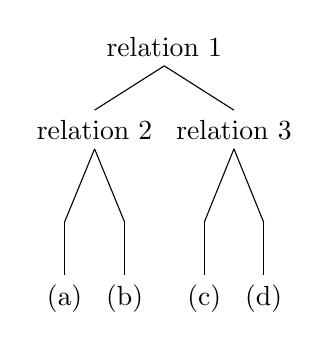
\begin{tikzpicture}
\Tree[.relation~1
       [.relation~2
         [ (a) ]
         [ (b) ]
       ]
       [.relation~3
         [ (c) ]
         [ (d) ]
       ]
     ]

\end{tikzpicture}

\caption{\label{i:rst-tree} A discourse sub-tree. }
\end{figure}


Comparatively, the Penn Discourse Treebank 2.0 (PDTB2)~\citep{Prasad08thepenn}
is a much larger corpus. The annotations were done on 2,159 articles from
the WSJ corpus of the Penn Treebank~\citep{marcus1993building}. They adopted a lexically-grounded
approach, annotating explicit relations signalled by connectives without constructing higher-level
structures as done in RST-DT. Therefore, the arguments do not span over long ranges. In fact,
more than 90\% of the arguments appear in the same sentence of the connective or the
exact immediately preceding sentence as pointed out by \cite{kong2014a}.
In addition, they annotated implicit relations for successive pairs of sentences.


\section{English Discourse Researches}

Many groups have investigated different subtasks of English
discourse parsing on PDTB2. \cite{pitler2009using} trained a maximum
entropy classifier with various syntactic features to identify explicit discourse
connectives and achieved the F1 of 94.19\%. Additionally, they used
a Naive Bayes classifier to classify the relation type of each connective and
achieved the accuracy of 94.15\%. Such high performance was already comparable to human
annotator agreement. They have found that the degree of relation type ambiguity
for connectives are low in English. In fact, an accuracy of 93.67\% can be achieved
by using the strings of connectives as the only features. \cite{wellner2009sequence}
also experimented with constituency-based and dependency-based features to identify
explicit connectives with logistic regression classifier. In addition, they proposed
a sequential ranking model to jointly identify discourse connectives and their arguments.
They developed a dependency-based discourse parsing system. \cite{faiz2013identifying} combined
various feature sets to improve the results on connective identification. \cite{j2013disambig} pointed
out that while a few connectives constitute most of connective instances, most articles contain
at least one low-frequency connective. Therefore, using macro-average over different connectives
may be a better metric. They also showed that simple lexical features such as POS tags perform
well in this experimental setting when golden standard parsing tree is not available.

\cite{dines2005attribution} used a tree subtraction algorithm to extract arguments for
intra-sentential subordinating conjunctions. \cite{wellner2007auto} considered the task of identifying
arguments for discourse connectives. They used a log-linear ranking model to extract the heads of arguments.
\cite{elwell2008discourse} followed the work to identify the heads and showed that
interpolating connective specific models with general models can improve performance.
\cite{ghosh2011shallow,ghosh2012global} formulated the problem as sequence labelling task
and used Conditional Random Fields (CRFs) to tackle the problem.
\cite{kong2014a} developed a constituent-based approach to extract arguments.
\cite{lin2014pdtb} build an end-to-end discourse parser for PDTB2.


As RST-DT provides hierarchy discourse structure annotations. There are also many
attempts to construct these discourse structures automatically. \cite{soricut2003sentence}
investigated sentence-level discourse parsing. They built discourse segmenter to
segment each sentence into EDUs using a statistical model with lexical and syntactic features.
They evaluated the model by the ability to recover EDU boundaries and achieved the F1 of
83.1\% with automatically generated parsing tree and 84.7\% with golden truth parsing tree.
They also constructed a discourse parser and showed that near-human level performance can be achieved
if golden truth syntactic parsing tree and EDU segmentation were given. \cite{sporleder2005} focused
on non-hierarchical discourse chunking and produced comparable results without the use of
syntactic parsers. \cite{fisher2007utility} investigated whether the features derived from finite-state
systems are enough for discourse segmentation and showed that combining features from syntactic tree
can improve the performance. \cite{joty2012novel} applied an CYK-like parsing algorithm
to sentence-level discourse parsing. By avoiding a greedy approach, they were able to increase
their performance.

Though sentence-level discourse parsing is well studied, document-level discourse
parsing still needs investigation. \cite{hernault2010hilda} attempted
document-level discourse parsing using Support Vector Machine (SVM) to
predict the discourse relations and construct the discourse tree in
a bottom-up fashion. \cite{feng2012text} further improved the results using more
linguistic features. \cite{joty2013combining} utilized CRFs to tackle this problem.
\cite{li2014recursive} experimented with a deep learning approach.
They recursively learn the representations for discourse units
while building the discourse tree in a bottom-up manner.


\section{Chinese Discourse Corpora}

There have been few Chinese discourse corpora compared to English until recently.
\cite{xue2005annotating} discussed the issues involved in annotating Chinese texts. They
pointed out the difficulty to determine argument spans due to the hierarchical
discourse structure. \cite{huang2011chinese} annotated 81 articles selected from
the Sinica Treebank 3.1~\footnote{http://turing.iis.sinica.edu.tw/treesearch/}. They followed
the top-level categories in PDTB for relation types and focused on the annotation
of inter-sentential discourse relations. \cite{huang2014interpretation} annotated the
relation types for 7,601 sentences that have only two discourse units.
\cite{zhou2012pdtb,zhou2015the} adopted PDTB-style discourse annotations and constructed
a Chinese discourse corpus that contains 164 articles selected from the \textit{Chinese
Treebank (CTB)}~\citep{xue2005penn}. \cite{zhang2014chinese} annotated 525 texts selected
from OntoNotes Release 4.0~\citep{weischedel_ontonotes_2011}. They have annotated
intra-sentential, inter-sentential, and passage-level relations, though
these annotations do not form a hierarchical structure naturally. \cite{zhou2014the}
refined the annotation scheme of PDTB2 and annotated 890 documents from CTB.
They focused mainly on intra-sentential discourse relations.

\cite{li2014building} proposed a \textit{Connective-driven Dependency Tree (CDT)}
scheme, which was designed specifically for Chinese rhetorical structure. They
annotated 500 documents from CTB. Each paragraph was segmented into EDUs similar
to the RST scheme. A three-level hierarchy of relation types was
proposed, and the explicit and implicit relations between different spans of EDUs
were annotated. The relations for each paragraph form a tree structure. In addition,
they annotated the discourse connectives for each relation. We use this corpus
for our study as it have both discourse connective annotations and discourse
structure annotations. We will discuss this corpus further in Section~\ref{s:CDTB}.

\section{Chinese Discourse Researches}


\cite{t1999applying,t2000enhancement} and \cite{chan2000mining} investigated
connective detection in Chinese texts as a part of a tagging system. \cite{hu2009research}
developed a fully automatic system to extract connective components from sentences.
They used a rule-based method and found that the performance was sensitive to
the connective lexicon. By removing words commonly used in non-discourse contexts,
they were able to improve accuracy from 58.66\% to 89.88\%.
\cite{zhou2012cross} and \cite{li2014cross} employed
cross-lingual information to deal with discourse usage ambiguity.
Their reported F scores are 79.33\% and 71.63\%, respectively.
\cite{li2014cross} used 5-way classification to classify a connective
between four relation types and non-discourse usage,
and obtained overall accuracy of 70.20\%. \cite{li2015automatic} use CDTB to
investigate detection and classification of connective components. They use
maximum entropy and decision tree algorithms with various syntactic features.
The best F1 for connective identification as 69.2\% and the best classification
accuracy among four top-level relation types was 89.1\%.

\cite{hu2011research} dealt with linking ambiguity. They focused on sentences
that have multiple clauses and assumed all connective components in the sentence
are correctly identified. They developed a method to prune the search tree
to avoid the computation of all solutions while trying to find a connective
set that includes all connective components. They were able to achieve 98.9\%
accuracy in the 79 sentences that have linking ambiguities.

\cite{huang2011chinese} investigated relation type disambiguation between
two sentences. They used four-class classification with SVM, and their reported
accuracy and macro-average F1 are 88.28\% and 63.69\% respectively.
\cite{huang2012contingency} dealt with intra-sentential relations identification
and tackled the relation structure prediction with a 49-way classification
between different types of relation structures in a sentence.

%
%   Chapter Datasets
%
%   Yong-Siang Shih
%   R.O.C.104.07
%
\chapter{Datasets}
\label{c:datasets}

In this chapter, we discuss the datasets we use in our study, and
provide some statistics and analysis.

\section{Chinese Discourse Treebank (CDTB)}
\label{s:CDTB}
\subsection{Introduction}

Chinese Discourse Treebank (CDTB)~\citep{li2014building} is a discourse
corpus that contains 500 articles from the Chinese Treebank (CTB)~\citep{xue2005penn}.
Totally, it contains 2,342 paragraphs.
Inspired by RST and PDTB, they proposed the Connective-driven Dependency Tree (CDT)
scheme to annotate the documents.

In CDTB, each paragraph is represented as a discourse tree. The leaf nodes are the
elementary discourse units (EDUs) for the text, while internal nodes are discourse
relations between discourse units. This is very similar to RST-DT.

The set of discourse relation types is organized in a three-level hierarchy as
shown in Figure~\ref{i:three-level}.
The top-level categories have four relation types including causality, coordination,
transition, and explanation. The second level
have 17 types. The third level are the discourse connectives themselves.
As some connectives may be used for different relation types, there may
be multiple third-level connectives that have the same surface form under
different second-level relation types. For example, the connective
``并'' (and) appear in the following second-level relation types:
progressive, continue, explanation, coordination.

% i:three-level
\begin{figure}[!htbp]
\begin{multicols}{2}
\begin{itemize}
  \item[] \textbf{causality}
  \begin{itemize}
    \item cause-result 
    \begin{itemize}
      \item[-] because \ldots
    \end{itemize}
    \item inference
    \begin{itemize}
      \item[-] so that \ldots
    \end{itemize}
    \item hypothetical
    \begin{itemize}
      \item[-] if \ldots
    \end{itemize}
    \item purpose
    \begin{itemize}
      \item[-] in order to \ldots
    \end{itemize}
    \item condition
    \begin{itemize}
      \item[-] only \ldots
    \end{itemize}
    \item background
    \begin{itemize}
      \item[-] background \ldots
    \end{itemize}
  \end{itemize}

  \item[] \textbf{transition}
  \begin{itemize}
    \item transition
    \begin{itemize}
      \item[-] but \ldots
    \end{itemize}
    \item concessive
    \begin{itemize}
      \item[-] although \ldots
    \end{itemize}
  \end{itemize}

  \vfill
  \columnbreak

  \item[] \textbf{coordination}
  \begin{itemize}
    \item coordination
    \begin{itemize}
      \item[-] and \ldots
    \end{itemize}
    \item continue
    \begin{itemize}
      \item[-] first \ldots second \ldots
    \end{itemize}
    \item progressive
    \begin{itemize}
      \item[-] in addition \ldots
    \end{itemize}
    \item selectional
    \begin{itemize}
      \item[-] or \ldots
    \end{itemize}
    \item inverse
    \begin{itemize}
      \item[-] compared with \ldots
    \end{itemize}
  \end{itemize}

  \item[] \textbf{explanation}
  \begin{itemize}
    \item explanation
    \begin{itemize}
      \item[-] which including \ldots
    \end{itemize}
    \item summary-elaboration
    \begin{itemize}
      \item[-] in a word \ldots
    \end{itemize}
    \item example
    \begin{itemize}
      \item[-] e.g. \ldots
    \end{itemize}
    \item evaluation
    \begin{itemize}
      \item[-] evaluation \ldots
    \end{itemize}
  \end{itemize}
\end{itemize}
\end{multicols}

\caption{\label{i:three-level} A three-level set of discourse relations in
CDTB. }
\end{figure}


For an explicit relation, once its second-level type is determined, the
third-level type is just its explicit connective. For an implicit relation,
a connective that could be inserted is annotated as its third-level type.
Sometimes there is no appropriate connective to be inserted. In that case,
the relation is only annotated with a second-level relation type.

Consider the example sentences (S~\ref{sent:cdtb}) from CDTB. Its discourse
structure are shown in Figure~\ref{i:cdtb-tree}. The continue relation between
discourse units (a-b) and (c) is implicit, but ``以后'' (later) can be inserted
as a connective as denoted by ``<以后>'' in (S~\ref{sent:cdtb}).
On the other hand, the explanation relation between (d) and (e-g)
does not have an inserted connective.


\begin{sent}{sent:cdtb}{}
    [\underline{尽管}浦东新区制定的法规性文件有些比较``粗'',]\textsuperscript{a}
    [有些\underline{还}只是暂行规定,]\textsuperscript{b}
    [有待<以后>在实践中逐步完善,]\textsuperscript{c}
    [\underline{但}这种法制紧跟经济和社会活动的做法,]\textsuperscript{d}
    [受到了国内外投资者的好评,]\textsuperscript{e}
    [他们认为,到浦东新区投资办事有章法,]\textsuperscript{f}
    [讲规矩,]\textsuperscript{g}
    [利益能得到保障。]\textsuperscript{h}

    (Although some regulatory documents for the Pudong New Area are "rough",
    and some regulations are still temporary and
    need to be refined gradually,
    the practice for regulations to closely follow economic and social activities
    are praised by domestic and foreign investors.
    Their view on investing in the Pudong New Area is that
    things are done methodologically,
    rules are followed,
    and their interest can be protected.)
\end{sent}

% i:cdtb-tree
\begin{figure}[!htbp]
\centering
\tikzset{every tree node/.style={align=center},
    level distance=40pt,
    sibling distance=6pt}
\begin{tikzpicture}
\Tree[.{concessive \\ 尽管 \ldots 但 (although \ldots but)}
       [.{continue \\ (以后) (later)}
         [.{coordination \\ 还 (still)}
           [ (a) ]
           [ (b) ]
         ]
         [ (c) ]
       ]
       [.{explanation}
         [ (d) ]
         [.{coordination}
           [ (e) ]
           [ (f) ]
           [ (g) ]
         ]
       ]
     ]

\end{tikzpicture}

\caption{\label{i:cdtb-tree} A discourse tree in CDTB. }
\end{figure}


Since we only consider explicit relations in our studies, we will ignore
third-level relation types from now on to avoid confusion.
For an explicit relation, the second-level relation type and its explicit
connective can already uniquely determine its relation type.
When we refer to connective classes in the following section, we mean the
surface forms of connectives (i.e. instances of the same connective class
may have different relation types).

\subsection{Analysis}

During our experiments, we found some errors in the corpus including
duplicate annotations and erroneous positions, so we corrected
them. After the correction, there are 2,131 connective component instances
annotated for the explicit relations, and they form 1,813 connective instances.
The length distribution for the connectives are shown in Table~\ref{t:connective-length}.
The distribution is imbalance. Most connectives only have
one or two connective components. Also, while some connectives have many instances,
many connectives appear rarely. The frequencies for the connectives are shown
in Figure~\ref{i:freq}. There are totally 274 classes of connectives, but
147 of them only appear once.

% t:connective-length
\begin{table}[ht]
\centering
\begin{tabular}{|c|c|c|c|c|c|c|}
\hline
\bf \#Components        & 1    & 2   & 3  & 4 & 6 & 7 \\ \hline
\bf \#Connective Types  & 143  & 108 & 15 & 6 & 1 & 1 \\ \hline
\bf \#Instances         & 1544 & 235 & 24 & 8 & 1 & 1 \\ \hline
\end{tabular}
\caption{\label{t:connective-length} Lengths of connectives.}
This tables shows how many connective types have a specific length
and how many instances they totally appear. The number of types
is counted by the surface forms for the connectives.
\end{table}


% i:freq
\begin{figure}[!htbp]
\centering
    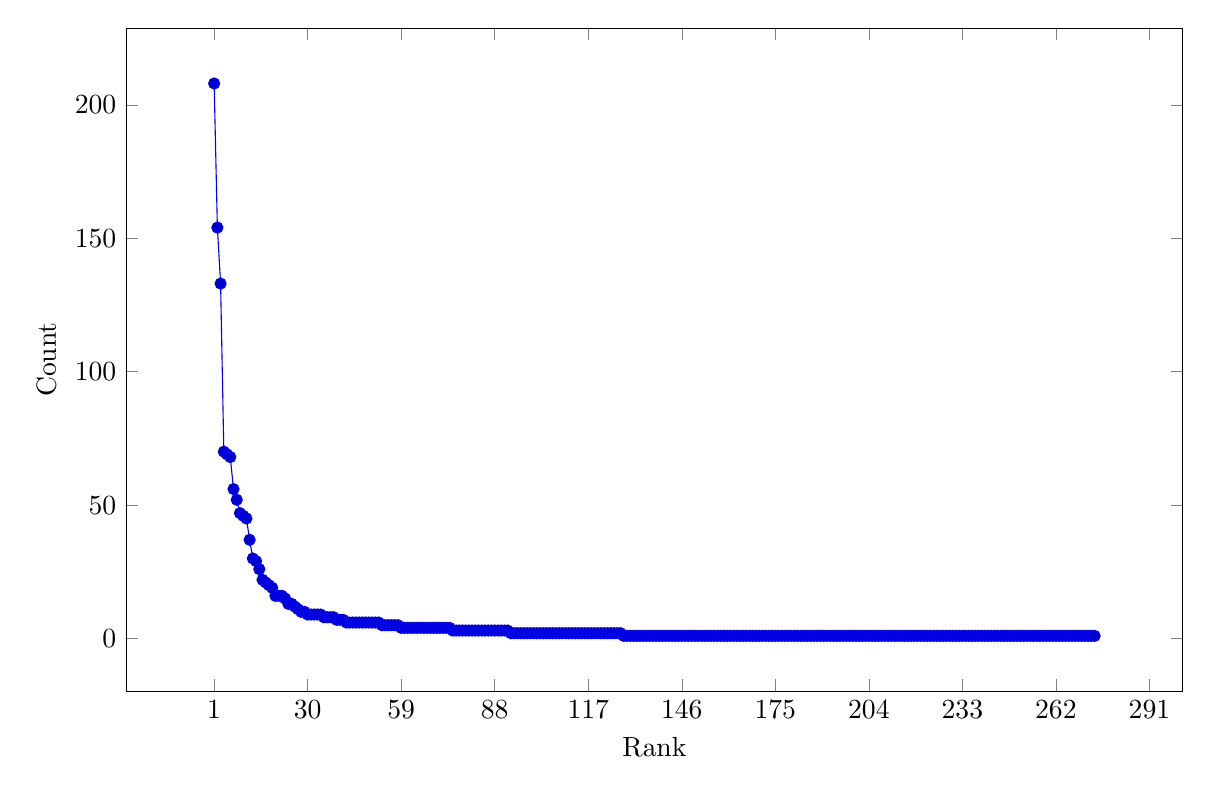
\begin{tikzpicture}
        \begin{axis}[
                width=15cm,
                height=10cm,
                xlabel=Rank,
                ylabel=Count,
                xtick={1,30,...,262,291},
                xticklabel style={/pgf/number format/assume math mode},
                yticklabel style={/pgf/number format/assume math mode},
            ]

            \addplot+[sharp plot] coordinates
            {
            (1,208)
            (2,154)
            (3,133)
            (4,70)
            (5,69)
            (6,68)
            (7,56)
            (8,52)
            (9,47)
            (10,46)
            (11,45)
            (12,37)
            (13,30)
            (14,29)
            (15,26)
            (16,22)
            (17,21)
            (18,20)
            (19,19)
            (20,16)
            (21,16)
            (22,16)
            (23,15)
            (24,13)
            (25,13)
            (26,12)
            (27,11)
            (28,10)
            (29,10)
            (30,9)
            (31,9)
            (32,9)
            (33,9)
            (34,9)
            (35,8)
            (36,8)
            (37,8)
            (38,8)
            (39,7)
            (40,7)
            (41,7)
            (42,6)
            (43,6)
            (44,6)
            (45,6)
            (46,6)
            (47,6)
            (48,6)
            (49,6)
            (50,6)
            (51,6)
            (52,6)
            (53,5)
            (54,5)
            (55,5)
            (56,5)
            (57,5)
            (58,5)
            (59,4)
            (60,4)
            (61,4)
            (62,4)
            (63,4)
            (64,4)
            (65,4)
            (66,4)
            (67,4)
            (68,4)
            (69,4)
            (70,4)
            (71,4)
            (72,4)
            (73,4)
            (74,4)
            (75,3)
            (76,3)
            (77,3)
            (78,3)
            (79,3)
            (80,3)
            (81,3)
            (82,3)
            (83,3)
            (84,3)
            (85,3)
            (86,3)
            (87,3)
            (88,3)
            (89,3)
            (90,3)
            (91,3)
            (92,3)
            (93,2)
            (94,2)
            (95,2)
            (96,2)
            (97,2)
            (98,2)
            (99,2)
            (100,2)
            (101,2)
            (102,2)
            (103,2)
            (104,2)
            (105,2)
            (106,2)
            (107,2)
            (108,2)
            (109,2)
            (110,2)
            (111,2)
            (112,2)
            (113,2)
            (114,2)
            (115,2)
            (116,2)
            (117,2)
            (118,2)
            (119,2)
            (120,2)
            (121,2)
            (122,2)
            (123,2)
            (124,2)
            (125,2)
            (126,2)
            (127,2)
            (128,1)
            (129,1)
            (130,1)
            (131,1)
            (132,1)
            (133,1)
            (134,1)
            (135,1)
            (136,1)
            (137,1)
            (138,1)
            (139,1)
            (140,1)
            (141,1)
            (142,1)
            (143,1)
            (144,1)
            (145,1)
            (146,1)
            (147,1)
            (148,1)
            (149,1)
            (150,1)
            (151,1)
            (152,1)
            (153,1)
            (154,1)
            (155,1)
            (156,1)
            (157,1)
            (158,1)
            (159,1)
            (160,1)
            (161,1)
            (162,1)
            (163,1)
            (164,1)
            (165,1)
            (166,1)
            (167,1)
            (168,1)
            (169,1)
            (170,1)
            (171,1)
            (172,1)
            (173,1)
            (174,1)
            (175,1)
            (176,1)
            (177,1)
            (178,1)
            (179,1)
            (180,1)
            (181,1)
            (182,1)
            (183,1)
            (184,1)
            (185,1)
            (186,1)
            (187,1)
            (188,1)
            (189,1)
            (190,1)
            (191,1)
            (192,1)
            (193,1)
            (194,1)
            (195,1)
            (196,1)
            (197,1)
            (198,1)
            (199,1)
            (200,1)
            (201,1)
            (202,1)
            (203,1)
            (204,1)
            (205,1)
            (206,1)
            (207,1)
            (208,1)
            (209,1)
            (210,1)
            (211,1)
            (212,1)
            (213,1)
            (214,1)
            (215,1)
            (216,1)
            (217,1)
            (218,1)
            (219,1)
            (220,1)
            (221,1)
            (222,1)
            (223,1)
            (224,1)
            (225,1)
            (226,1)
            (227,1)
            (228,1)
            (229,1)
            (230,1)
            (231,1)
            (232,1)
            (233,1)
            (234,1)
            (235,1)
            (236,1)
            (237,1)
            (238,1)
            (239,1)
            (240,1)
            (241,1)
            (242,1)
            (243,1)
            (244,1)
            (245,1)
            (246,1)
            (247,1)
            (248,1)
            (249,1)
            (250,1)
            (251,1)
            (252,1)
            (253,1)
            (254,1)
            (255,1)
            (256,1)
            (257,1)
            (258,1)
            (259,1)
            (260,1)
            (261,1)
            (262,1)
            (263,1)
            (264,1)
            (265,1)
            (266,1)
            (267,1)
            (268,1)
            (269,1)
            (270,1)
            (271,1)
            (272,1)
            (273,1)
            (274,1)
                };
        \end{axis}
    \end{tikzpicture}
\caption{\label{i:freq} Frequencies of connectives. }
\end{figure}



We list the top 25 classes of connectives in Figure~\ref{i:connective-types}.
Most of these connectives have only one component.

% i:connective-types
\begin{figure}[ht]
\centering
    \begin{tikzpicture}
        \begin{axis}[
            width=15cm,
            bar width = 7pt,
            enlarge x limits=0.05,
            symbolic x coords={
            并, 其中, 也, 而, 但, 还, 使, 以, 为, 同时,
            后, 由于, 因此, 如, 又, 为了, 因为, 而且, 如果, 後,
            此外, 虽然-但, 但是, 从而, 然而
            }, 
            ybar,
            nodes near coords,
            x tick label style={font=\small,align=center,rotate=70},
            xtick=data
          ]
            \addplot[ybar,fill=blue] coordinates {
                (并,  208)
                (其中,    154)
                (也,  133)
                (而,  70)
                (但,  69)
                (还,  68)
                (使,  56)
                (以,  52)
                (为,  47)
                (同时,    46)
                (后,  45)
                (由于,    37)
                (因此,    30)
                (如,  29)
                (又,  26)
                (为了,    22)
                (因为,    21)
                (而且,    20)
                (如果,    19)
                (後,  16)
                (此外,    16)
                (虽然-但, 16)
                (但是,    15)
                (从而,    13)
                (然而,    13)
            };
        \end{axis}
    \end{tikzpicture}
\caption{\label{i:connective-types} Top 25 Types. }
\end{figure}


While there are totally 274 classes of connectives, there are only 227 classes
of connective components found in the explicit relation annotations. This
is because many components can either be a single connective or link
with other components to form a parallel connective. We collect these
connectives and connective components to construct a connective lexicon
that has 274 entries and a component lexicon that has 227 entries.


Although many connectives appear rarely, there exist many spurious connective
candidates that do not actually have discourse meaning. This can be seen in
Figure~\ref{i:freq-detected}. We show the number of connective candidates
detected if we use string matching with the connective lexicon to extract
all connective candidates from the corpus. This problem is partly caused by the linking
ambiguities but the large number of spurious component candidates is a worse problem.
These spurious component candidates introduce a lot of connective candidates that
do not actually have discourse meanings. In fact, if we could identify the correct
connective components, the total number of connective candidates they form
is only 2,249, and 1,813 of them are correct, which is about 80\% of these candidates.

% i:freq-detected
\begin{figure}[ht]
\centering
    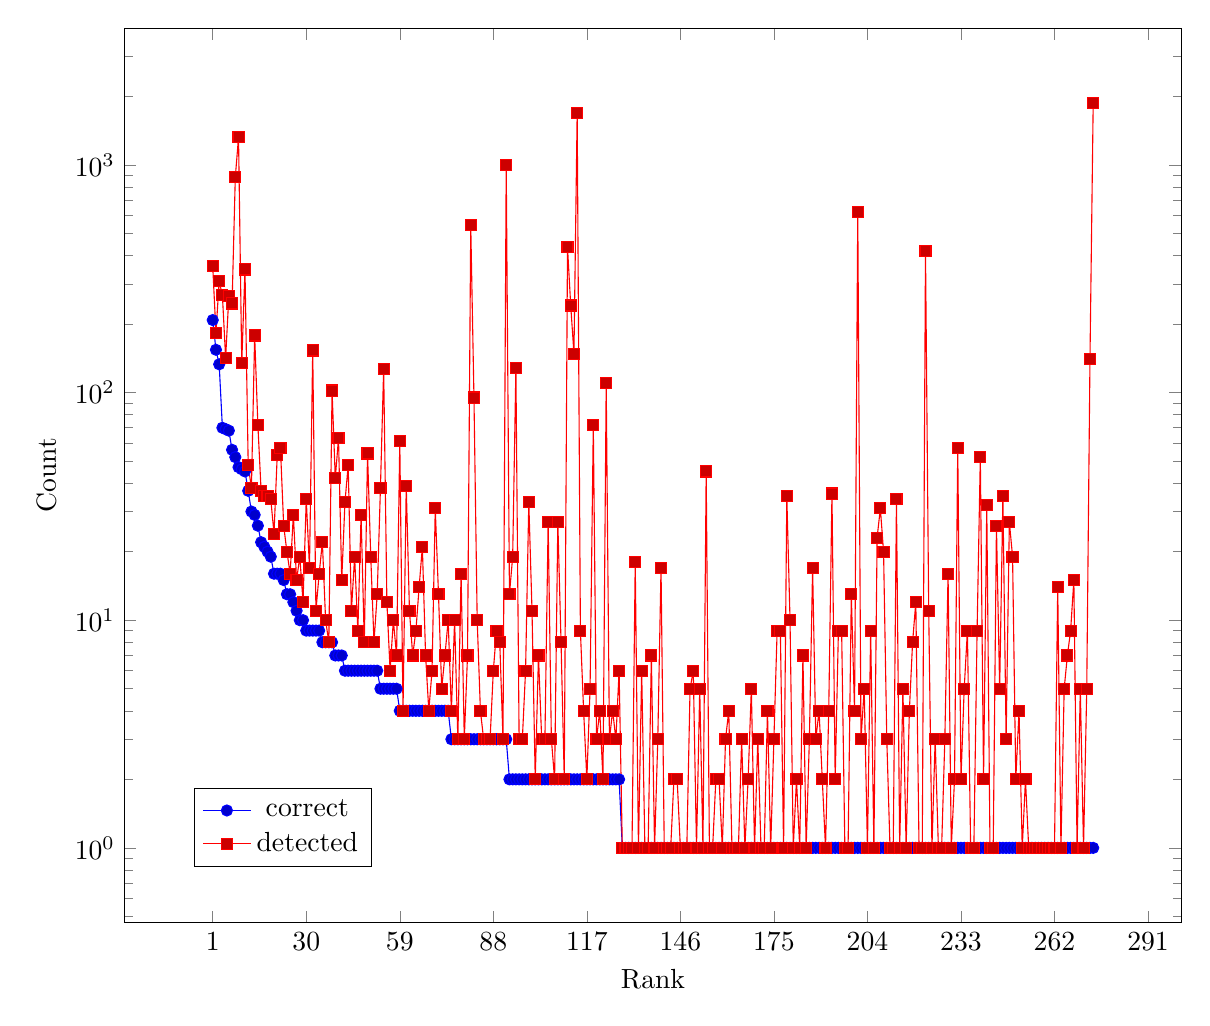
\begin{tikzpicture}
        \begin{axis}[
                width=15cm,
                xlabel=Rank,
                ylabel=Count,
                legend style={at={(0.15,0.15)},
                anchor=north},
                xtick={1,30,...,262,291},
                ymode=log,
            ]

            \addplot+[sharp plot] coordinates
            {
            (1,208)
            (2,154)
            (3,133)
            (4,70)
            (5,69)
            (6,68)
            (7,56)
            (8,52)
            (9,47)
            (10,46)
            (11,45)
            (12,37)
            (13,30)
            (14,29)
            (15,26)
            (16,22)
            (17,21)
            (18,20)
            (19,19)
            (20,16)
            (21,16)
            (22,16)
            (23,15)
            (24,13)
            (25,13)
            (26,12)
            (27,11)
            (28,10)
            (29,10)
            (30,9)
            (31,9)
            (32,9)
            (33,9)
            (34,9)
            (35,8)
            (36,8)
            (37,8)
            (38,8)
            (39,7)
            (40,7)
            (41,7)
            (42,6)
            (43,6)
            (44,6)
            (45,6)
            (46,6)
            (47,6)
            (48,6)
            (49,6)
            (50,6)
            (51,6)
            (52,6)
            (53,5)
            (54,5)
            (55,5)
            (56,5)
            (57,5)
            (58,5)
            (59,4)
            (60,4)
            (61,4)
            (62,4)
            (63,4)
            (64,4)
            (65,4)
            (66,4)
            (67,4)
            (68,4)
            (69,4)
            (70,4)
            (71,4)
            (72,4)
            (73,4)
            (74,4)
            (75,3)
            (76,3)
            (77,3)
            (78,3)
            (79,3)
            (80,3)
            (81,3)
            (82,3)
            (83,3)
            (84,3)
            (85,3)
            (86,3)
            (87,3)
            (88,3)
            (89,3)
            (90,3)
            (91,3)
            (92,3)
            (93,2)
            (94,2)
            (95,2)
            (96,2)
            (97,2)
            (98,2)
            (99,2)
            (100,2)
            (101,2)
            (102,2)
            (103,2)
            (104,2)
            (105,2)
            (106,2)
            (107,2)
            (108,2)
            (109,2)
            (110,2)
            (111,2)
            (112,2)
            (113,2)
            (114,2)
            (115,2)
            (116,2)
            (117,2)
            (118,2)
            (119,2)
            (120,2)
            (121,2)
            (122,2)
            (123,2)
            (124,2)
            (125,2)
            (126,2)
            (127,2)
            (128,1)
            (129,1)
            (130,1)
            (131,1)
            (132,1)
            (133,1)
            (134,1)
            (135,1)
            (136,1)
            (137,1)
            (138,1)
            (139,1)
            (140,1)
            (141,1)
            (142,1)
            (143,1)
            (144,1)
            (145,1)
            (146,1)
            (147,1)
            (148,1)
            (149,1)
            (150,1)
            (151,1)
            (152,1)
            (153,1)
            (154,1)
            (155,1)
            (156,1)
            (157,1)
            (158,1)
            (159,1)
            (160,1)
            (161,1)
            (162,1)
            (163,1)
            (164,1)
            (165,1)
            (166,1)
            (167,1)
            (168,1)
            (169,1)
            (170,1)
            (171,1)
            (172,1)
            (173,1)
            (174,1)
            (175,1)
            (176,1)
            (177,1)
            (178,1)
            (179,1)
            (180,1)
            (181,1)
            (182,1)
            (183,1)
            (184,1)
            (185,1)
            (186,1)
            (187,1)
            (188,1)
            (189,1)
            (190,1)
            (191,1)
            (192,1)
            (193,1)
            (194,1)
            (195,1)
            (196,1)
            (197,1)
            (198,1)
            (199,1)
            (200,1)
            (201,1)
            (202,1)
            (203,1)
            (204,1)
            (205,1)
            (206,1)
            (207,1)
            (208,1)
            (209,1)
            (210,1)
            (211,1)
            (212,1)
            (213,1)
            (214,1)
            (215,1)
            (216,1)
            (217,1)
            (218,1)
            (219,1)
            (220,1)
            (221,1)
            (222,1)
            (223,1)
            (224,1)
            (225,1)
            (226,1)
            (227,1)
            (228,1)
            (229,1)
            (230,1)
            (231,1)
            (232,1)
            (233,1)
            (234,1)
            (235,1)
            (236,1)
            (237,1)
            (238,1)
            (239,1)
            (240,1)
            (241,1)
            (242,1)
            (243,1)
            (244,1)
            (245,1)
            (246,1)
            (247,1)
            (248,1)
            (249,1)
            (250,1)
            (251,1)
            (252,1)
            (253,1)
            (254,1)
            (255,1)
            (256,1)
            (257,1)
            (258,1)
            (259,1)
            (260,1)
            (261,1)
            (262,1)
            (263,1)
            (264,1)
            (265,1)
            (266,1)
            (267,1)
            (268,1)
            (269,1)
            (270,1)
            (271,1)
            (272,1)
            (273,1)
            (274,1)
            };

            \addplot+[sharp plot] coordinates
            {
            (1,359)
            (2,183)
            (3,308)
            (4,267)
            (5,142)
            (6,265)
            (7,246)
            (8,883)
            (9,1321)
            (10,135)
            (11,347)
            (12,48)
            (13,38)
            (14,178)
            (15,72)
            (16,37)
            (17,35)
            (18,35)
            (19,34)
            (20,24)
            (21,53)
            (22,57)
            (23,26)
            (24,20)
            (25,16)
            (26,29)
            (27,15)
            (28,19)
            (29,12)
            (30,34)
            (31,17)
            (32,153)
            (33,11)
            (34,16)
            (35,22)
            (36,10)
            (37,8)
            (38,102)
            (39,42)
            (40,63)
            (41,15)
            (42,33)
            (43,48)
            (44,11)
            (45,19)
            (46,9)
            (47,29)
            (48,8)
            (49,54)
            (50,19)
            (51,8)
            (52,13)
            (53,38)
            (54,127)
            (55,12)
            (56,6)
            (57,10)
            (58,7)
            (59,61)
            (60,4)
            (61,39)
            (62,11)
            (63,7)
            (64,9)
            (65,14)
            (66,21)
            (67,7)
            (68,4)
            (69,6)
            (70,31)
            (71,13)
            (72,5)
            (73,7)
            (74,10)
            (75,4)
            (76,10)
            (77,3)
            (78,16)
            (79,3)
            (80,7)
            (81,545)
            (82,95)
            (83,10)
            (84,4)
            (85,3)
            (86,3)
            (87,3)
            (88,6)
            (89,9)
            (90,8)
            (91,3)
            (92,1000)
            (93,13)
            (94,19)
            (95,128)
            (96,3)
            (97,3)
            (98,6)
            (99,33)
            (100,11)
            (101,2)
            (102,7)
            (103,3)
            (104,3)
            (105,27)
            (106,3)
            (107,2)
            (108,27)
            (109,8)
            (110,2)
            (111,435)
            (112,241)
            (113,148)
            (114,1695)
            (115,9)
            (116,4)
            (117,2)
            (118,5)
            (119,72)
            (120,3)
            (121,4)
            (122,2)
            (123,110)
            (124,3)
            (125,4)
            (126,3)
            (127,6)
            (128,1)
            (129,1)
            (130,1)
            (131,1)
            (132,18)
            (133,1)
            (134,6)
            (135,1)
            (136,1)
            (137,7)
            (138,1)
            (139,3)
            (140,17)
            (141,1)
            (142,1)
            (143,1)
            (144,2)
            (145,2)
            (146,1)
            (147,1)
            (148,1)
            (149,5)
            (150,6)
            (151,1)
            (152,5)
            (153,1)
            (154,45)
            (155,1)
            (156,1)
            (157,2)
            (158,2)
            (159,1)
            (160,3)
            (161,4)
            (162,1)
            (163,1)
            (164,1)
            (165,3)
            (166,1)
            (167,2)
            (168,5)
            (169,1)
            (170,3)
            (171,1)
            (172,1)
            (173,4)
            (174,1)
            (175,3)
            (176,9)
            (177,9)
            (178,1)
            (179,35)
            (180,10)
            (181,1)
            (182,2)
            (183,1)
            (184,7)
            (185,1)
            (186,3)
            (187,17)
            (188,3)
            (189,4)
            (190,2)
            (191,1)
            (192,4)
            (193,36)
            (194,2)
            (195,9)
            (196,9)
            (197,1)
            (198,1)
            (199,13)
            (200,4)
            (201,622)
            (202,3)
            (203,5)
            (204,1)
            (205,9)
            (206,1)
            (207,23)
            (208,31)
            (209,20)
            (210,3)
            (211,1)
            (212,1)
            (213,34)
            (214,1)
            (215,5)
            (216,1)
            (217,4)
            (218,8)
            (219,12)
            (220,1)
            (221,1)
            (222,419)
            (223,11)
            (224,1)
            (225,3)
            (226,1)
            (227,1)
            (228,3)
            (229,16)
            (230,1)
            (231,2)
            (232,57)
            (233,2)
            (234,5)
            (235,9)
            (236,1)
            (237,1)
            (238,9)
            (239,52)
            (240,2)
            (241,32)
            (242,1)
            (243,1)
            (244,26)
            (245,5)
            (246,35)
            (247,3)
            (248,27)
            (249,19)
            (250,2)
            (251,4)
            (252,1)
            (253,2)
            (254,1)
            (255,1)
            (256,1)
            (257,1)
            (258,1)
            (259,1)
            (260,1)
            (261,1)
            (262,1)
            (263,14)
            (264,1)
            (265,5)
            (266,7)
            (267,9)
            (268,15)
            (269,1)
            (270,5)
            (271,1)
            (272,5)
            (273,140)
            (274,1873)
            };

            %\addplot+[sharp plot] coordinates
            %{
            %(1,212)
            %(2,154)
            %(3,182)
            %(4,85)
            %(5,110)
            %(6,106)
            %(7,57)
            %(8,53)
            %(9,47)
            %(10,61)
            %(11,49)
            %(12,41)
            %(13,36)
            %(14,30)
            %(15,39)
            %(16,24)
            %(17,24)
            %(18,31)
            %(19,31)
            %(20,18)
            %(21,27)
            %(22,18)
            %(23,22)
            %(24,18)
            %(25,13)
            %(26,13)
            %(27,13)
            %(28,10)
            %(29,10)
            %(30,9)
            %(31,16)
            %(32,12)
            %(33,9)
            %(34,9)
            %(35,8)
            %(36,8)
            %(37,8)
            %(38,8)
            %(39,9)
            %(40,7)
            %(41,8)
            %(42,7)
            %(43,13)
            %(44,6)
            %(45,6)
            %(46,6)
            %(47,10)
            %(48,6)
            %(49,6)
            %(50,11)
            %(51,6)
            %(52,8)
            %(53,5)
            %(54,8)
            %(55,5)
            %(56,6)
            %(57,6)
            %(58,6)
            %(59,13)
            %(60,4)
            %(61,4)
            %(62,5)
            %(63,5)
            %(64,6)
            %(65,4)
            %(66,5)
            %(67,5)
            %(68,4)
            %(69,4)
            %(70,16)
            %(71,6)
            %(72,4)
            %(73,6)
            %(74,6)
            %(75,3)
            %(76,5)
            %(77,3)
            %(78,5)
            %(79,3)
            %(80,4)
            %(81,5)
            %(82,8)
            %(83,4)
            %(84,4)
            %(85,3)
            %(86,3)
            %(87,3)
            %(88,6)
            %(89,4)
            %(90,4)
            %(91,3)
            %(92,4)
            %(93,3)
            %(94,5)
            %(95,2)
            %(96,2)
            %(97,2)
            %(98,6)
            %(99,2)
            %(100,2)
            %(101,2)
            %(102,2)
            %(103,2)
            %(104,2)
            %(105,3)
            %(106,3)
            %(107,2)
            %(108,3)
            %(109,2)
            %(110,2)
            %(111,2)
            %(112,2)
            %(113,2)
            %(114,2)
            %(115,2)
            %(116,2)
            %(117,2)
            %(118,2)
            %(119,3)
            %(120,2)
            %(121,2)
            %(122,2)
            %(123,6)
            %(124,2)
            %(125,2)
            %(126,2)
            %(127,4)
            %(128,1)
            %(129,1)
            %(130,1)
            %(131,1)
            %(132,3)
            %(133,1)
            %(134,4)
            %(135,1)
            %(136,1)
            %(137,6)
            %(138,1)
            %(139,1)
            %(140,3)
            %(141,1)
            %(142,1)
            %(143,1)
            %(144,1)
            %(145,1)
            %(146,1)
            %(147,1)
            %(148,1)
            %(149,1)
            %(150,1)
            %(151,1)
            %(152,1)
            %(153,1)
            %(154,1)
            %(155,1)
            %(156,1)
            %(157,2)
            %(158,1)
            %(159,1)
            %(160,1)
            %(161,1)
            %(162,1)
            %(163,1)
            %(164,1)
            %(165,3)
            %(166,1)
            %(167,1)
            %(168,2)
            %(169,1)
            %(170,1)
            %(171,1)
            %(172,1)
            %(173,1)
            %(174,1)
            %(175,1)
            %(176,1)
            %(177,1)
            %(178,1)
            %(179,1)
            %(180,1)
            %(181,1)
            %(182,1)
            %(183,1)
            %(184,1)
            %(185,1)
            %(186,2)
            %(187,3)
            %(188,1)
            %(189,1)
            %(190,1)
            %(191,1)
            %(192,2)
            %(193,1)
            %(194,1)
            %(195,2)
            %(196,1)
            %(197,1)
            %(198,1)
            %(199,13)
            %(200,1)
            %(201,1)
            %(202,1)
            %(203,1)
            %(204,1)
            %(205,1)
            %(206,1)
            %(207,1)
            %(208,1)
            %(209,2)
            %(210,3)
            %(211,1)
            %(212,1)
            %(213,1)
            %(214,1)
            %(215,1)
            %(216,1)
            %(217,1)
            %(218,2)
            %(219,1)
            %(220,1)
            %(221,1)
            %(222,1)
            %(223,6)
            %(224,1)
            %(225,2)
            %(226,1)
            %(227,1)
            %(228,1)
            %(229,1)
            %(230,1)
            %(231,1)
            %(232,1)
            %(233,2)
            %(234,1)
            %(235,1)
            %(236,1)
            %(237,1)
            %(238,1)
            %(239,1)
            %(240,1)
            %(241,2)
            %(242,1)
            %(243,1)
            %(244,2)
            %(245,1)
            %(246,3)
            %(247,1)
            %(248,14)
            %(249,1)
            %(250,1)
            %(251,1)
            %(252,1)
            %(253,1)
            %(254,1)
            %(255,1)
            %(256,1)
            %(257,1)
            %(258,1)
            %(259,1)
            %(260,1)
            %(261,1)
            %(262,1)
            %(263,1)
            %(264,1)
            %(265,2)
            %(266,3)
            %(267,4)
            %(268,5)
            %(269,1)
            %(270,3)
            %(271,1)
            %(272,1)
            %(273,1)
            %(274,5)
            %};
            %\legend{correct,detected,detected for correct components}
            \legend{correct,detected}
        \end{axis}
    \end{tikzpicture}
\caption{\label{i:freq-detected} Frequencies of annotated connectives vs. detected connectives. }
\end{figure}


The problem caused by spurious component candidates is best illustrated in
Figure~\ref{i:linking-ambig-chart}. When correct components are identified,
the connective candidates formed by these components are limited.
Most of the components involve in only one connective, meaning that the correct linking
is known. The greatest linking ambiguity is only 5. However, when there are
spurious components, there exist a component candidate that involves in as many
as 240 connective candidates.

% i:linking-ambig-chart
\begin{figure}[ht]
\centering
    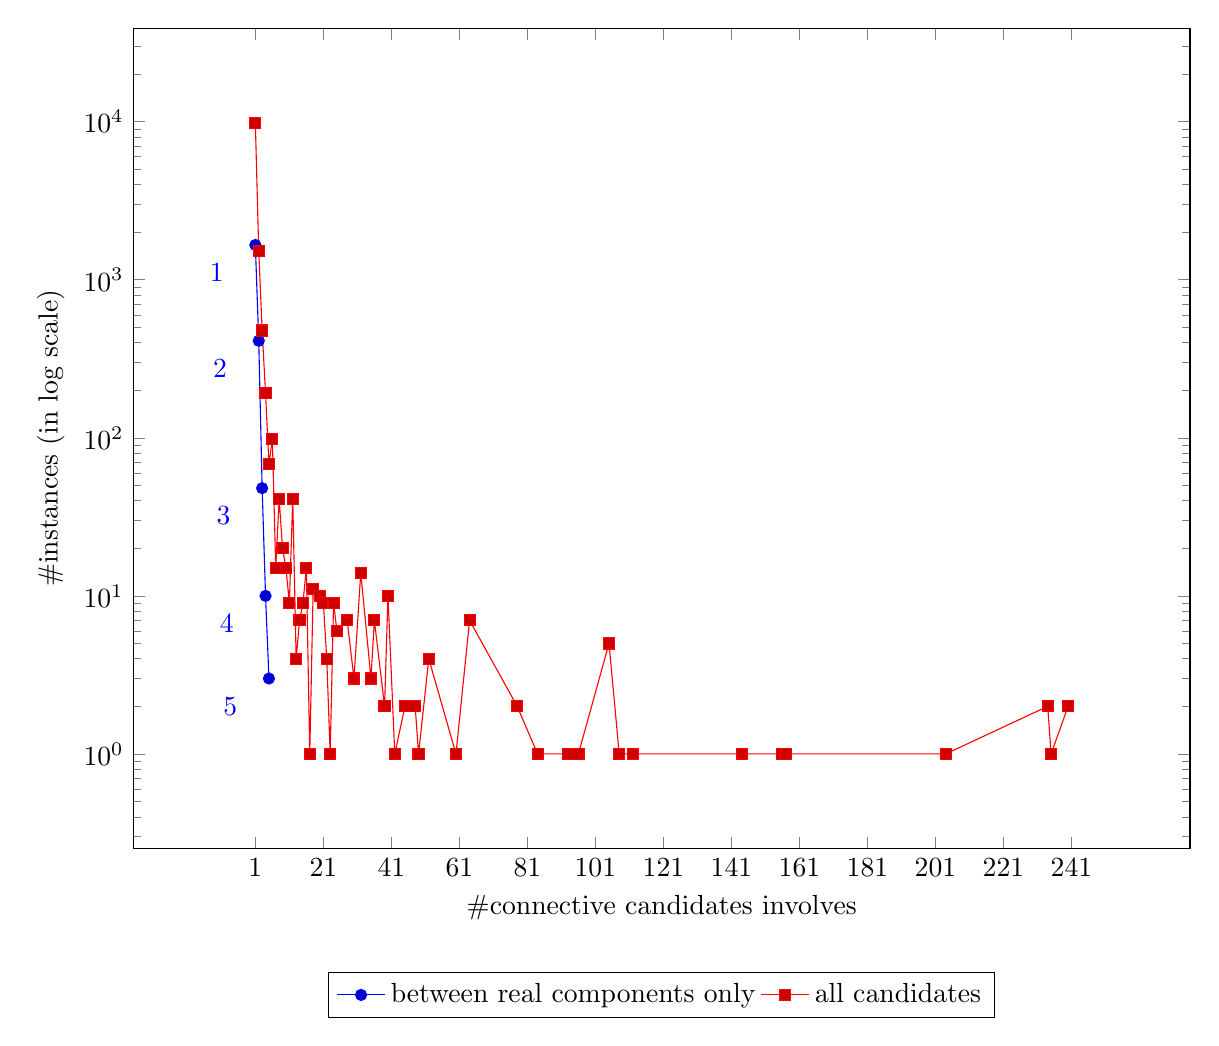
\begin{tikzpicture}
        \begin{axis}[
            width=15cm,
            height=12cm,
            enlargelimits=0.15,
            legend style={at={(0.5,-0.15)},
              anchor=north,legend columns=-1},
            xtick={1,21,...,245},
            xlabel={\#connective candidates involves},
            ylabel={\#instances (in log scale)},
            ymode=log,
            ]
        \addplot+[
                nodes near coords,
                every node near coord/.append style={xshift=-20, yshift=-10},
                nodes near coords align={horizontal},
                point meta=x,
                ] coordinates {
        (1,1659)
        (2,411)
        (3,48)
        (4,10)
        (5,3)
        };
        \addplot coordinates {
        (1,9827)
        (2,1525)
        (3,477)
        (4,191)
        (5,68)
        (6,98)
        (7,15)
        (8,41)
        (9,20)
        (10,15)
        (11,9)
        (12,41)
        (13,4)
        (14,7)
        (15,9)
        (16,15)
        (17,1)
        (18,11)
        (20,10)
        (21,9)
        (22,4)
        (23,1)
        (24,9)
        (25,6)
        (28,7)
        (30,3)
        (32,14)
        (35,3)
        (36,7)
        (39,2)
        (40,10)
        (42,1)
        (45,2)
        (48,2)
        (49,1)
        (52,4)
        (60,1)
        (64,7)
        (78,2)
        (84,1)
        (93,1)
        (96,1)
        (105,5)
        (108,1)
        (112,1)
        (144,1)
        (156,1)
        (157,1)
        (204,1)
        (234,2)
        (235,1)
        (240,2)
        };
        \legend{between real components only,all candidates}
        \end{axis}
    \end{tikzpicture}
\caption{\label{i:linking-ambig-chart} Number of connective candidates a component candidate involes. }
\end{figure}


For relation type ambiguity, we list the number of relation types a
connective used for explicit relations in the corpus in Table~\ref{t:connective-type}.
While most connective classes are only used for 1 relation type,
the ambiguous connectives have many instances.

% t:connective-type
\begin{table}[ht]
\centering
\begin{tabular}{|c|c|c|c|c|c|}
\hline
\#Top-level Relation Types & 1    & 2   & 3   & 4   & 5  \\ \hline
\#Connective Classes       & 258  & 15  & 1   & -   & -  \\ \hline
\#Instances                & 1388 & 355 & 70  & -   & -  \\

\hhline{|=|=|=|=|=|=|}

\#2nd-level Relation Types & 1    & 2   & 3   & 4   & 5  \\ \hline
\#Connective Classes       & 243  & 24  & 5   & 1   & 1  \\ \hline
\#Instances                & 1030 & 379 & 126 & 208 & 70 \\ \hline

\end{tabular}
\caption{\label{t:connective-type} Relation ambiguity of connectives. }
\end{table}


Table~\ref{t:argument-num} shows the number of arguments for the 1,813 explicit
relations. Most relations only have two arguments, but there are relations
that have as many as 7 arguments. The number of arguments does not always
match with the number of connective components in each relation. The same
connective can also have different number of arguments when used in
different relations. Single connectives can have as many as 6 arguments
as shown in (S~\ref{sent:same-time}), and in (S~\ref{sent:medal}),
the connective 除-外-还 (in addition to \ldots also)
has three components, but it only have two arguments.

% t:argument-num
\begin{table}[ht]
\centering
\begin{tabular}{|c|c|c|c|c|c|c|}
\hline

\#Arguments              & 2    & 3   & 4   & 5   & 6  & 7  \\ \hline
\#Instances              & 1688 & 85  & 33  & 4   & 2  & 1  \\ \hline

\end{tabular}
\caption{\label{t:argument-num} Number of arguments for each explicit relation. }
\end{table}


\begin{sent}{sent:same-time}{}
    [允许中资企业保留一定限额外汇收入,可以促使企业加强经济核算,]
    [降低生产经营成本,]
    [减少企业买卖外汇的支出,]
    [\underline{同时}可消除中外资企业在结汇方面的差别待遇,]
    [完善外汇市场运作和人民币汇率形成机制,]
    [扩大金融机构外汇存贷款业务。]
    (Allowing Chinese companies to retain a certain quota of foreign exchange earnings
     may encourage enterprises to enhance economic accounting.
     This reduces production and operation costs, and the expenses for foreign
     exchanges.  At the same time, it eliminates the different treatments between
     Chinese and foreign-funded enterprises in terms of foreign exchange settlement,
     improving the operation of the foreign exchange market and the RMB
     exchange rate formation mechanism, expanding the foreign currency deposits and
     loans of financial institutions.)
\end{sent}

\begin{sent}{sent:medal}{}
    [\underline{除}戈杰安夺得金牌\underline{外},]
    [米洛索维奇\underline{还}摘取铜牌。]
    (In addition to Gogean's gold medal, Milosovici also won the bronze medal.)
\end{sent}

\section{NTU PN-Gram Corpus}

NTU PN-Gram Corpus~\citep{yu2012development} is a large-scale corpus that was
constructed by POS-tagging the Chinese texts from the ClueWeb09
dataset~\citep{callan2009clueweb09}. In NTU PN-Gram, there are totally 173,741,587
web pages containing 141,179,769,123 tokens.

Recently, efficient methods to estimate word embeddings have been developed.
These methods learn the distributed representations for each word that encode
syntactic and semantic patterns for each word in a fixed-dimensional vector.
These vectors exhibit interesting properties. For example,
\cite{mikolov2013linguistic} pointed out that there exist linear regularities
between these vectors:

$$ vector('king') - vector('man') + vector('woman') \approx vector('queen') $$

Therefore, we investigate whether these vectors are useful for solving
discourse issues. Due to the limitation of computation powers, we use
a subset of NTU PN-Gram that was extracted by \cite{huang2014interpretation}
to train our word embeddings. These sentences were extracted with three conditions:

\begin{enumerate}
\item Each sentence must have exactly two clauses.
\item Each sentence must have exactly one instance of connective.
\item Each of the two clauses must not have more than 20 Chinese characters.
\end{enumerate}

We use an intermediate result that contains 43,010,050 sentences and eliminated
the duplicate sentences. The result are 21,217,147 sentences, containing
326,996,602 tokens. These sentences are used to train word embeddings.
We have created 400-dimensional embeddings by GloVe tool~\citep{pennington2014glove}
and word2vec tool~\citep{mikolov2013efficient,mikolov2013distributed} with
continuous skip-gram model and continuous bag-of-words model.
These vectors are used as features as discussed in Chapter~\ref{c:method}.

%
%   Chapter Methods
%
%   Yong-Siang Shih
%   R.O.C.104.07
%
\chapter{Methods}
\label{c:method}

\section{Overview}

In this chapter, we discuss our system design for Chinese discourse analysis.
Our study mainly focuses on the analysis of explicit relations.
The stages for the pipeline system are shown in Figure~\ref{i:system}.

%i:system
\begin{figure}[ht]
\centering
\tikzstyle{block} = [rectangle, draw, node distance=1.5cm,
    text width=20em, text centered, rounded corners, minimum height=3em]
\tikzstyle{line} = [draw, -latex']
\tikzstyle{cloud} = [draw, ellipse, node distance=1.5cm,
    minimum height=2em]
\tikzstyle{container} = [draw, rectangle, dashed, inner sep=0.8em]

\begin{tikzpicture}[node distance = 2cm, auto]
    % Place nodes
    \node [cloud] (paragraph) {paragraph};
    \node [block, below of=paragraph] (identify) {A. Identify connective component candidates};
    \node [block, below=1.6em of identify] (eliminate) {B1. Eliminate non-discourse usages on component or connective level};
    \node [block, below of=eliminate] (linking) {B2. Identify correct connectives};
    \node [container, fit=(eliminate) (linking)] (merge) {};
    \node [block, below=1.6em of linking] (types) {C. Disambiguate relation types};
    \node [block, below of=types ] (arguments) {D. Extract relation arguments};
    % Draw edges
    \path [line] (identify) -- (eliminate);
    \path [line] (eliminate) -- (linking);
    \path [line] (linking) -- (types);
    \path [line] (types) -- (arguments);
    \path [line,dashed] (paragraph) -- (identify);
\end{tikzpicture}

\caption{\label{i:system} System overview. }
\end{figure}


Firstly, we extract connective component candidates from each paragraph.
Secondly, a classifier is used to disambiguate between discourse and
non-discourse usages for these component candidates. We then try to identify
the correct connectives by resolving the linking ambiguity between the remaining
component candidates.
A different approach that eliminates non-discourse usages and disambiguates
linkings both on the connective level is also experimented. The alternative
approaches are illustrated in Figure~\ref{i:system-B}.
Finally, we determine the relation types for each explicit
connective and extract the arguments for each relation.

%i:system-B
\begin{figure}[ht]
\centering
\tikzstyle{block} = [rectangle, draw, node distance=1.5cm,
    text width=10em, text centered, rounded corners, minimum height=3em]
\tikzstyle{line} = [draw, -latex']
\tikzstyle{cloud} = [draw, ellipse, node distance=1.5cm,
    minimum height=2em]
\tikzstyle{container} = [draw, rectangle, dashed, inner sep=0.8em]

\begin{tikzpicture}[node distance = 2cm, auto]
    % Place nodes
    \node [cloud] (components) {component candidates};

    \path (components)+(-2.5,-2)
        node [block] (eliminate1) {B1. Eliminate non-discourse components};

    \node [block, right=3em of eliminate1] (generate2) {B2. Generate all connective candidates};

    \node [block, below of=generate2] (eliminate2) {B2. Eliminate unlikely connective candidates};

    \node [block, below of=eliminate1] (generate1) {B1. Generate all connective candidates};

    \path (generate1)+(2.5,-2) node [block] (linking) {C. Resolve linking ambiguities};

    \node [cloud, below of=linking] (connectives) {connectives};

    % Draw edges
    \path [line] (eliminate1) -- (generate1);
    \path [line] (generate1) -- (linking);
    \path [line] (generate2) -- (eliminate2);
    \path [line] (eliminate2) -- (linking);
    \path [line,dashed] (linking) -- (connectives);
    \path [line,dashed] (components) -- (eliminate1);
    \path [line,dashed] (components) -- (generate2);
\end{tikzpicture}

\caption{\label{i:system-B} System overview for alternative methods
to extract connectives. } In B1, we eliminate non-discourse components first,
and generate all possible candidates by linking the components. In B2,
we do not eliminate components, but use all possible connective candidates, and
disambiguate discourse usages on the connective level. In fact, by eliminating
unlikely connective candidates, B2 actually solves some of linking ambiguities
before feeding the remaining candidates to C.
\end{figure}



\section{Connective Candidate Extraction}

\subsection{Goal}

To identify the correct discourse connectives, we need to
extract connective candidates and distinguish between discourse
and non-discourse usages among these candidates. Therefore, we tackle the
candidate identification first. In particular, we focus on the identification
of potential connective components, since connective candidates can then be
generated by forming links between these component candidates.

\subsection{Extraction Methods}

Given the input of a Chinese paragraph and the connective component lexicon we collected,
we would like to extract all possible positions of component candidates.
The simplest method is to just use string matching with the connective
component lexicon to extract all possible instances. This yields
24,539 candidates, while only 2,131 of them are correct instances. An improvement
could be made by making the observation that many of the components only have
discourse meaning when they are paired with other components. So instead of matching
with the connective component lexicon, we use connective lexicon and only extract
a component candidate when it could independently form a single connective or pair
with other candidates to form a parallel connective.
This leaves us with 12,498 candidates.

One reason for many incorrect instances is that many characters used for connectives
appear in other unrelated words. For example, even though ``如'' (if) is a connective,
this character appears in an unrelated word ``如是说'' (says). To alleviate this problem,
Stanford Chinese segmenter~\citep{chang2008optimizing} is employed to segment paragraphs
into tokens. The boundaries of these tokens can be used as clues for eliminating spurious candidates.
In particular, we only extract a component when it can be composed of complete tokens.
For example, in (S~\ref{sent:keyissue}) we extract ``不是'' (not) and ``而是'' (but) as candidates
even though ``不'' (not) and ``是'' (is) are separated. Comparatively, in (S~\ref{sent:peace}),
the spurious connective component candidate ``和'' (and) is not extracted because it does
not satisfy a token boundary.

\begin{sent}{sent:keyissue}{}
    当前 / 经济 / 的 / 关键 / \underline{不} / \underline{是} / 争取 / 更 /
    高 / 的 / 增长 / 速度 / , / \underline{而是} / 提高 / 效益 / 。
    (The key issue for current economy is not to pursue faster growth, but to
    increase productivity.)
\end{sent}

\begin{sent}{sent:peace}{}
    双方 / 表示 / 希望 / 在 / \underline{和}平 / 计划 / 的 / 基础 / 上 / 解决 / 问题 / 。
    (Both sides expressed the hope to solve the problem on the basis of the peace plan.)
\end{sent}

Using this procedure, only 7,649 component candidates are extracted, with 2,068 of 2,131 annotated
components recovered. These candidates could form 7,976 connective candidates, recovering
1,755 of 1,813 annotated connectives. Thus, 0.9704 and 0.9680 become upper bounds of recall
for the subsequent stages. Table~\ref{t:cand-extract} shows the comparison between different
extraction methods. The technique we use reduces the number of spurious candidates substantially while
maintaining high recall.

%t:cand-extract
\begin{table}[ht]
\centering
\begin{tabular}{|c|c|c|c|}
\hline
Method                  & component lexicon & connective lexicon & +segmentation \\ \hline

Component Recall        & 1                 & 1                  & 0.9704        \\ \hline
Component Precision     & 0.0868            & 0.1705             & 0.2704        \\

\hhline{|=|=|=|=|}

Connective Recall       & 1                 & 1                  & 0.9680        \\ \hline
Connective Precision    & 0.1196            & 0.1196             & 0.2200        \\ \hline

\end{tabular}
\caption{\label{t:cand-extract} Comparison between different candidate extraction methods.}
\end{table}


\section{Discourse Usage Disambiguation}
\label{s:discourse-disambig}

\subsection{Goal}

We start by investigating the identification of connective components that have discourse functions
as most of the related works also deal with connective components only.
Given the positions of all component candidates, we would like to eliminate spurious candidates.

\subsection{Disambiguation on Component Level}
\label{s:discourse-disambig-component}


We use \textit{Scikit-Learn} library~\citep{scikit-learn} to carry out binary
classification between discourse and non-discourse usages for all candidates.
Features for each connective component are extracted as specified in
Section~\ref{s:comp-features} and various
classifiers such as \textit{Logistic Regression} and
\textit{Support Vector Machine (SVM)}\footnote{The SVM included by Scikit-Learn is
a \textit{Python} wrapper for the popular \textit{LibSVM} library~\citep{CC01a}.}
have been experimented. The results are reported in Chapter~\ref{c:exp}. 
After we eliminate spurious components, we could form connective candidates
by linking the remaining components. Linking ambiguities must be resolved to
identify the correct connective afterwards.


\subsection{Features for a Connective Component Candidate}
\label{s:comp-features}

In this section we discuss the features we propose for each connective
component candidate.
Stanford POS tagger~\citep{toutanova2003feature} and Stanford Chinese
parser~\citep{levy2003harder} are used to create the POS tags and parsing trees
for the paragraphs. When we extract features related to the parsing tree, we use
utilities provided by the \textit{Natural Language Toolkit}~\citep{BirdKleinLoper09}
to manipulate the parsing trees. The features we used for classification
are as follows.

\subsubsection{P\&N}

The feature set is a subset of the features from
\cite{pitler2009using}. It includes four binary features:
(1) the highest category that dominates exactly the component
itself in the parsing tree, which is called self-category, (2) the parent of the self-category,
(3) the left-sibling of the self-category, and (4) the right-sibling of the self-category.
Special null features are set when no such nodes exist. For example,
in Figure~\ref{i:parse-but}, there is no node that dominates exactly the
connective component ``却是'' (but), while in Figure~\ref{i:parse-therefore} the
self-category of ``因此'' (therefore) is ADVP. We have also experimented
with the full feature set from \cite{pitler2009using}, but the performance
does not increase.

%i:parse-but
%i:parse-therefore
\begin{figure}[ht]

\begin{minipage}[b]{.5\textwidth}
  \centering
  \vspace{16pt}
  \Tree[.IP [.VP [.ADVP [.AD 却 ]]
                 [.VP [.VC 是 ]
                      [.PU 「 ]
                      [.NP [.NN 完了 ]]]]]
  \caption{\label{i:parse-but} A sub-parsing tree for 却是. }
\end{minipage}%
\begin{minipage}[b]{.5\textwidth}
  \centering
  \vspace{0pt}
  \Tree[.VP [.ADVP [.AD 因此 ]]
            [.PP [.P 对 ]
                 [.NP [.NN 地球 ]]]
            [.VP [.VE 无 ]
                 [.NP [.ADJP [.JJ 直接 ]]
                      [.NP [.NN 影响 ]]]]]
  \caption{\label{i:parse-therefore} A sub-parsing tree for 因此. }
\end{minipage}

\end{figure}


\subsubsection{POS}

The feature set contains three types of binary features:
(1) part-of-speech tags for all tokens that constitute the connective component,
(2) part-of-speech tag of the token to the left of the component, and
(3) part-of-speech tag of the token to the right of the component. For example,
in (S~\ref{sent:sovereignty}) the features for ``意味着'' (meaning) are
\textbf{POS-left-PU}, \textbf{POS-right-PN}, \textbf{POS-self-VV}, and
\textbf{POS-self-AS}.

\begin{sent}{sent:sovereignty}{}
    一百二十七/CD 位/M 委员/NN 一致/AD 通过/VV ,/PU \underline{意味/VV 着/AS} 大家/PN 对/P
    恢复/VV 行使/VV 香港/NR 主权/NN \underline{后/LC} 的/DEG 政治/NN 架构/NN 重建/NN ,/PU
    有/VE 着/AS 高度/JJ 的/DEG 共识/NN 。/PU
    (All 127 committee members agreed, meaning that everyone reaches a consensus about
    the reconstruction of political structure after resuming exercise of sovereignty over Hong Kong.)
\end{sent}

\subsubsection{NUM}

The feature set contains three numerical features.

\begin{enumerate}
    \item The number of detected connective candidates the component involves. The larger
        the number means that the component candidate can form more plausible connective
        candidates by linking with other component candidates.
    \item The distance from the connective component to a separating element on the left.
    \item The distance from the connective component to a
        separating element on the right.
\end{enumerate}

Distance is measured by adding 1 to the number of tokens
between the separating element and the nearest token of the component.
The separating elements include the symbols ``!?:;,。''.
When no such symbol is found, we use the distance to paragraph boundary.

For example, in (S~\ref{sent:sovereignty}) the features for “意味着” (meaning) are \textbf{NUM-ambiguity=1},
\textbf{NUM-left=1}, and \textbf{NUM-right=12}. As there is only one connective candidate that has the
component “意味着” (meaning), the linking ambiguity for the component is 1.
We normalize the numerical features by scaling each to zero mean and unit variance.


\subsubsection{VECTOR}

This feature set is built using word embeddings we created.
We have tried creating 400-dimensional embeddings by GloVe tool~\citep{pennington2014glove}
and word2vec tool~\citep{mikolov2013efficient,mikolov2013distributed}.

The vectors are used to construct three features: (1) the averaged vectors
for the tokens that constitute the connective component, (2) the vector for the
token to the left and (3) the vector for the token to the right. Zero-valued vector is used
when the vector does not exist.

In total, it's a 1200-dimensional vector when the 400-dimensional embeddings are used.
The dimensionality increases proportionally if we combine different vectors produced by
different tools.

\subsection{Disambiguation on Connective Level}
\label{s:discourse-disambig-connective}


Rather than disambiguate each component candidate, we could also treat each connective
candidate as an instance and tackle discourse usage disambiguation on the connective
level. All possible connective candidates are  generated by linking components with
each other. Features for each connective candidate are extracted as specified in
Section~\ref{s:connective-features} and binary
classification can be carried out to identify discourse usages.
Since there are more spurious connectives than real connectives, we balance the
data set by oversampling the correct instances for three times when training. To evaluate on
component level, we take the union of the components for all connective as the result.

By eliminating unlikely connective candidates, some linking ambiguities 
are also removed. In fact, if we can classify perfectly, we would have already
solved the linking ambiguities completely as only the correct connectives remain.
However, there may still exist some spurious candidates, some of which are
caused by incorrect component candidates, others caused by
incorrect linkings.
In particular, some overlapped connective candidates that share the same
connective component candidate remain. By resolving the linking
ambiguities, we will have more capacity to identify the correct connectives. This
work is described in Section~\ref{s:linking-disambig}.

\subsection{Features for a Connective Candidate}
\label{s:connective-features}

The feature sets for each connective candidate are similar to those in the previous
experiment. As a connective candidate is composed of one or more component candidates,
we extend some of the features to utilize linking relationships between the
components.

\subsubsection{P\&N}

The feature set contains the union of self-category, parent-category, left-sibling,
and right-sibling as defined in Section~\ref{s:comp-features} for each component.
For example, in Figure~\ref{i:parse-although}, the features for ``虽'' (although) are
\textbf{PN-self-ADVP}, \textbf{PN-parent-VP}, \textbf{PN-left-Null}, and \textbf{PN-right-ADVP}, while
the features for ``但'' (but) are \textbf{PN-self-ADVP}, \textbf{PN-parent-IP}, \textbf{PN-left-Null},
and \textbf{PN-right-NP}. Therefore, the combined features for ``虽-但'' (although-but) are
\textbf{PN-self-ADVP}, \textbf{PN-parent-VP}, \textbf{PN-parent-IP}, \textbf{PN-left-Null},
\textbf{PN-right-ADVP}, and \textbf{PN-right-NP}.


%i:parse-although
\begin{figure}[ht]
\centering
\begin{tikzpicture}
\Tree[.IP [.IP [.NP [.NR 台湾 ]]
               [.VP [.ADVP [.CS 虽 ]]
                    [.ADVP [.AD 只 ]]
                    [. ... ]]]
          [.PU , ]
          [.IP [.ADVP [.AD 但 ]]
               [.NP [.ADJP [.JJ 後续 ]]
                    [.NP      [.NN 冲击 ]]]
               [.VP [.ADVP [.AD 将 ]]
                    [.QP [.CD 一 ]
                         [.CLP [.M 波波 ]]]
                    [.VP [.VV 涌到 ]]]]]
\end{tikzpicture}
\caption{\label{i:parse-although} A sub-parsing tree for 虽-但. }
\end{figure}

%                    [.VP [.VV 遭 ]
%                    [.NP [.NN 风暴 ]
%                         [.NN 边缘 ]
%                         [.NN 扫过 ]]]]]



\subsubsection{POS}

The feature set contains three types of binary features:
(1) part-of-speech tags for all tokens that constitute the connective components
of the connective candidate,
(2) part-of-speech tag of the token to the left of each component, and
(3) part-of-speech tag of the token to the right of each component. For example,
in (S~\ref{sent:crisis}), the features for ``虽-但'' (although-but) are
\textbf{POS-left-NR}, \textbf{POS-right-AD}, \textbf{POS-self-CS},
\textbf{POS-left-PU}, \textbf{POS-right-JJ}, and \textbf{POS-self-AD}.

\begin{sent}{sent:crisis}{}
    东亚/NR 诸国/NN 宛如/VV 骨牌/NN 般/VA 连番/AD 倒下/VV 。/PU
    台湾/NR \underline{虽/CS} 只/AD 遭/VV 风暴/NN 边缘/NN 扫过/VV ,/PU
    \underline{但/AD} 後续/JJ 冲击/NN 将/AD 一/CD 波波/M 涌到/VV 。/PU
    (East Asian countries fell like dominoes.
    Although Taiwan is only swept by the edge of the storm,
    the follow-up impact would come.)
\end{sent}

\subsubsection{NUM}

The feature set contains the length of the connective as a set
of binary features. The length is defined as the number of components
that it contains.
In additional, there are seven numerical features.
\begin{enumerate}
    \item The number of overlapped connective candidates. Any connective
        candidates that share a token with any of the components for the current
        candidate are considered as overlapped.
    \item The number of connective candidates that cross any
        components of the current connective. A connective crosses a component
        if the component is between any two components of the connective.
    \item The distance between the leftmost and the rightmost tokens of the connective.
        The distance is measured by tokens as before.
    \item The geometric mean of distances between all neighboring connective components for
        the current connective candidates.
    \item The distances from the leftmost connective component to a separating element on the left.
    \item The distance from the rightmost connective component to a separating element on the right.
    \item The minimum distance from any separating element to any connective component.
\end{enumerate}

The separating elements include the symbols ``!?:;,。''.
When no such symbol is found, we use the distance to paragraph boundary.
We normalize the numerical features by scaling each to zero mean and unit variance.

\subsubsection{VECTOR}

This feature set is built using word embeddings as before, averaging over all components.
In particular, it contains three vectors: (1) the averaged vectors
for the all tokens that constitute each connective component the connective candidate has,
(2) the averaged vector for the
token to the left of each component and (3) the averaged vector for the token to the
right of each component. Zero-valued vector is used when the vector does not exist.

\section{Connective Linking Disambiguation}
\label{s:linking-disambig}

\subsection{Goal}

Depending on the method we choose for discourse usage disambiguation, we
either have a set of connective component candidates or a set of connective
candidates. Given all component candidates, we could construct all possible
connective candidates formed by these components by linking them together.
Many of these candidates are incorrect. In particular, a component may involves in
multiple different connective candidates by linking with different components,
but only one of them could be correct. Moreover, some remaining component
candidates may not actually have discourse usage, meaning that none of
the connectives it forms is correct. We would like to extract the
correct connectives from the paragraph despite the imperfect discourse usage
disambiguation.

\subsection{A Greedy Algorithm}

We propose a greedy algorithm to resolve linking ambiguities among a set of
connective candidates as outlined in Algorithm~\ref{a:linking-resolve}.
The algorithm filters the candidate set $C$ and produces a result set $A$ that
contains only non-overlapped connective candidates. On line~\ref{a:lnk:compute}
and \ref{a:lnk:check}, the algorithm computes the number of connective candidates
each component candidate involves in the remaining $C$, and checks if there exists
a component that does not have multiple possible linkings. When such a candidate
is not found, we rank all connective candidates under some criteria
and select the one with the highest priority.

As we will see in our experiments, accepting components that have no ambiguity
is especially helpful when the only task is to resolve linking ambiguities among
component candidates that are known to be correct.
In fact, under this condition, we can guarantee the connective candidate
$c_i$ found on line~\ref{a:lnk:select} is correct as long as $A$ does not yet have
any spurious connective candidates. Moreover, one could also develop a non-greedy
algorithm that guarantees to produce a result set that contains all component
candidates as done by \cite{hu2011research}. However, we consider that not knowing
which component candidate is correct is a more realistic experiment setting so
we will not go into that direction.

\begin{algorithm}
    \caption{Linking Resolution Algorithm}
    \label{a:linking-resolve}
    \begin{algorithmic}[1]
        \Require
            $C$: A set of connective candidates
        \Ensure
            $A$: A set of accepted connectives
        \State $A \gets \{\}$
        \Comment{Initialize $A$}
        \While{$C$ is not empty }
            \State Compute linking ambiguities for all connective components exist in $C$ \label{a:lnk:compute}
            \If{there exists a connective component $ cc_i $ that has linking ambiguity $=$ 1} \label{a:lnk:check}
                \State let $ c_i $ be the unique connective candidate the component involves \label{a:lnk:select}
            \Else
                \State Rank all connective candidates in $ C $
                \State let $ c_i $ be the connective candidate that have highest priority
            \EndIf
                \State $C \gets C - \{c_i\}$
                \State $A \gets A \cup \{c_i\}$
            \State Remove all connective candidates $ c_j \in C $ that overlap with $ c_i $
        \EndWhile
        \State \Return A
    \end{algorithmic}
\end{algorithm}

When we use Algorithm~\ref{a:linking-resolve} in a pipeline system,
there exist many component candidates in $C$ that do not have discourse meaning,
and accepting any component that has linking ambiguity $=$ 1 could easily
introduce many spurious connective candidates. Therefore, we would just rank all
candidates and use their priority to greedily accept candidates. The simplified
algorithm is outlined in Algorithm~\ref{a:linking-rank}.

\begin{algorithm}
    \caption{Linking Resolution Algorithm by Ranking Only}
    \label{a:linking-rank}
    \begin{algorithmic}[1]
        \Require
            $C$: A set of connective candidates
        \Ensure
            $A$: A set of accepted connectives
        \State $A \gets \{\}$
        \Comment{Initialize $A$}
        \State Rank all connective candidates in $ C $
        \While{$C$ is not empty }
            \State let $ c_i $ be the connective candidate that have highest priority
            \State $C \gets C - \{c_i\}$
            \State $A \gets A \cup \{c_i\}$
            \State Remove all connective candidates $ c_j \in C $ that overlap with $ c_i $
        \EndWhile
        \State \Return A
    \end{algorithmic}
\end{algorithm}

We will use different ranking criteria to evaluate our models. The experiments are
explained in Section~\ref{s:linking-exp}.

\begin{description}
\item[Score] We use the features described in Section~\ref{s:connective-features} to
    train a logistic regression classifier to predict whether a connective candidate
    has discourse meaning and use the probability obtained as its score.

\item[Length] We use the number of components each connective candidate has as its
    score. This is based on our observation: when a component candidate can
    pair with other components, it's less likely for it to be a single connective by
    itself.

\item[Position] The positions of the components a connective candidate has is used
    as a tie-breaker for the ranking algorithm. In particular, we accept the left-most
    candidate first.
\end{description}

We explain two alternative pipeline approaches that correspond to two different
discourse usage disambiguation as described in Section~\ref{s:discourse-disambig-component}
and \ref{s:discourse-disambig-connective}.

\subsubsection{A Pipeline Approach with Discourse Usage Disambiguation on Component Level}
\label{s:pipeline1}

After we have eliminated the non-discourse connective components as described
in Section~\ref{s:discourse-disambig-component}, we could
deal with liking ambiguities by determining how to correctly pair these
components together. We generate all possible connective candidates by
linking these components. These candidates form a candidate set $ C $ and the set is
fed to the linking resolving algorithm to obtain the final result $ A $.
To obtain the scores, we treat each candidate as an instance to
extract the related features as described in Section~\ref{s:connective-features}.
Afterwards, logistic regression is used to obtain the likelihood for a
candidate to be a correct connective.

After this procedure, additional connective components may have been eliminated if
they are unable to form a link with other candidates and is not a single connective.
Therefore, we also evaluate whether this procedure could improve the performance
for discourse usage identification on component level.


\subsubsection{A Pipeline Approach with Discourse Usage Disambiguation on Connective Level}
\label{s:pipeline2}

Rather than eliminating non-discourse connective components first and
dealing with linking disambiguation for overlapped connectives later,
we could also try to solve them both on connective level as linking may
provide additional clues for detecting discourse usage. 

In Section~\ref{s:discourse-disambig-component}, we generate all possible
connective candidates and eliminate the ones that are unlikely to be correct.
In the process, we eliminate some non-discourse candidates and some incorrect
linkings.

Afterwards, there remain some connective candidates that overlap with each other.
That is, they share the same connective component. So we feed these candidates
to the linking resolving algorithm to obtain the final result. Since each candidate
already has a predicted score when disambiguating the discourse usage, the score
is used directly.

Likewise, we also evaluate on component level to see if this increases
the performance for discourse usage detection.

\section{Relation Type Disambiguation}

After the connectives are extracted, the relation type each connective represents
must be determined. Different classifiers are used to investigate whether the features in
Section~\ref{s:connective-features} are useful for relation type disambiguation.
Additionally, we also use the string of the connective as a feature as it provides strong
clues for the connective's relation type.

\section{Connective Argument Extraction}

\subsection{Goal}

After the connective and its relation type is identified, we would like to extract
its arguments. For example, in Figure~\ref{i:cdtb-tree2}, the discourse tree
for (S~\ref{sent:rare-earth}) is shown. There exist two explicit relations signalled by
connectives ``其中'' (among them) and ``并'' (and). We would like to know the
arguments for ``其中'' (among them) are (b) and (c) while arguments for ``并'' (and) are
(d), (e), (f), (g) and (h).

%i:cdtb-tree2
\begin{figure}[!htbp]
\centering
\tikzset{every tree node/.style={align=center},
    level distance=40pt,
    sibling distance=6pt}
\begin{tikzpicture}
\Tree[.explanation
       [ (a) ]
       [.{coordination\textsuperscript{*}}
         [.{summary-elaboration \\ 其中 (among them)}
           [ (b) ]
           [ (c) ]
         ]
         [.{coordination\textsuperscript{+} \\ 并 (and)}
           [ (d) ]
           [ (e) ]
           [ (f) ]
           [ (g) ]
           [ (h) ]
         ]
       ]
     ]

\end{tikzpicture}

\caption{\label{i:cdtb-tree2} A discourse tree. }
\end{figure}


\begin{sent}{sent:rare-earth}{}
    [科技攻关带动了包头稀土工业生产的迅速发展。]\textsuperscript{a}
    [现已建成包钢稀土一、二、三厂等稀土生产厂家,]\textsuperscript{b}
    [\underline{其中}有世界最大的稀土精矿、稀土合金生产厂。]\textsuperscript{c}
    [目前包头可以生产八十多种稀土产品,]\textsuperscript{d}
    [这些产品以其独特的优良性能畅销全国,]\textsuperscript{e}
    [\underline{并}出口十几个国家和地区,]\textsuperscript{f}
    [年产值和利税达二十多亿元和三亿多元,]\textsuperscript{g}
    [出口值达五千多万美元。]\textsuperscript{h}
    (Science and technology research led to the rapid development of industrial production
    for rare earth minerals in Baotou. Baotou Steel Rare Earth has now completed three
    plants for rare earth production. Among them are the world's largest rare earth
    concentrate and rare earth alloy production plant. Baotou can now produce more than
    eighty kinds of rare earth products. With its excellent properties, these products
    are sold nationwide and exported to more than 10 countries and regions.
    The annual output value and profit tax is more
    than two billion yuan and three hundred million yuan, respectively.
    The export value is more than fifty million US dollars.)
\end{sent}

\subsubsection{Argument Extraction as a Sequence Labelling Problem}

We could formulate argument extraction as a sequence labelling problem.
Figure~\ref{i:rare-args} shows the arguments and the corresponding labels
for the four relations in Figure~\ref{i:cdtb-tree2}. Though we will
focus on explicit relations, the implicit relations are also shown
for completeness.
As we know the arguments will span over a continuous interval,
we use four labels for the EDUs: \textit{before}, \textit{start},
\textit{inside}, \textit{after}. Each argument is represented by
a \textit{start} followed by zero or more \textit{inside}s.

%i:rare-args
\begin{figure}[!htbp]
\centering

explanation
\[
\begin{array}{*8{c}}
(a)&(b)&(c)&(d)&(e)&(f)&(g)&(h)\\[-2pt]
\downarrow&\downarrow&\downarrow&\downarrow&\downarrow&\downarrow&\downarrow&\downarrow\\[-2pt]
\undermat{arg1}{start}&\undermat{arg2}{start&inside&inside&inside&inside&inside&inside}
\end{array}
\]
\vspace{1em}

coordination\textsuperscript{*}
\[
\begin{array}{*8{c}}
(a)&(b)&(c)&(d)&(e)&(f)&(g)&(h)\\[-2pt]
\downarrow&\downarrow&\downarrow&\downarrow&\downarrow&\downarrow&\downarrow&\downarrow\\[-2pt]
before&\undermat{arg1}{start&inside}&\undermat{arg2}{start&inside&inside&inside&inside}
\end{array}
\]
\vspace{1em}

summary-elaboration
\[
\begin{array}{*8{c}}
(a)&(b)&(c)&(d)&(e)&(f)&(g)&(h)\\[-2pt]
\downarrow&\downarrow&\downarrow&\downarrow&\downarrow&\downarrow&\downarrow&\downarrow\\[-2pt]
before&\undermat{arg1}{start}&\undermat{arg2}{start}&after&after&after&after&after
\end{array}
\]
\vspace{1em}

coordination\textsuperscript{+}
\[
\begin{array}{*8{c}}
(a)&(b)&(c)&(d)&(e)&(f)&(g)&(h)\\[-2pt]
\downarrow&\downarrow&\downarrow&\downarrow&\downarrow&\downarrow&\downarrow&\downarrow\\[-2pt]
before&before&before&\undermat{arg1}{start}&\undermat{arg2}{start}&\undermat{arg3}{start}&\undermat{arg4}{start}&\undermat{arg5}{start}
\end{array}
\]
\vspace{1em}

\caption{\label{i:rare-args} Sequence labeling for relation arguments. }

\end{figure}


To obtain the correct labels, one must first segment the paragraph
into EDUs and then classify each EDU for a particular label.
However, as our goal is to extract the arguments, only the
argument boundaries must be determined as shown in
Figure~\ref{i:rare-bounds}. For a relation that has $N$ arguments,
there are $N+1$ boundaries. As long as we can identify these boundaries,
we could extract the arguments.


%i:rare-bounds
\begin{figure}[ht]
\centering

summary-elaboration
\[
\begin{array}{*{11}{c}}
(a)& &(b)& &(c)& &(d)&(e)&(f)&(g)&(h)\\[-2pt]
\downarrow& &\downarrow& &\downarrow& &\downarrow&\downarrow&\downarrow&\downarrow&\downarrow\\[-2pt]
before& &\undermat{arg1}{start}& &\undermat{arg2}{start}& &after&after&after&after&after\\
&\downarrow& &\downarrow& &\downarrow& & & & & \\
&\bullet& &\bullet& &\bullet& & & & &
\end{array}
\]

\caption{\label{i:rare-bounds} Determination of boundaries for arguments. }

\end{figure}


Therefore, it's not required to obtain the EDUs as long as
we can divide the paragraph into segments that include all these boundaries.
In fact, even if we simply use the tokens as the segments, we could still satisfy
this requirement. One could improve the segmentation by making the observation
that the EDU boundaries in CDTB only occur with certain symbols that separate
phrases and sentences. The symbols include ”, …, ─, 、, 。, 」, !, ,, :, ; and ?.
We would segment the paragraph by these symbols, and solve the sequence labelling
problem on these segments.

\subsection{Determination of Argument Boundaries}

We use Conditional Random Fields (CRFs) to solve the sequence labelling problem.
The implementation we use is CRFsuite~\citep{CRFsuite}. When training, each explicit
relation with its corresponding labelling is used as an training case. When testing,
CRFs are used to label the segments for each connective we extracted. Therefore,
the same segments for a paragraph is labelled independently for each explicit relation
inside the paragraph. The resulting argument boundaries are used to extract the connective's
arguments. Although we have tried some rule-based techniques to adjust the argument boundaries
after they are extracted by utilizing their hierarchical relationships,
no significant improvement was observed.

\subsection{Features for a Segment}

In this section, we discuss the features we use for each segment.

\subsubsection{CONTEXT}

This feature set is similar to the P \& N features, but we relax the
definition of self-category since most segments do not have a node that
dominates exactly its tokens. For each segment, we find the lowest node
that dominates all of the tokens in the segment. It may additionally
dominates some tokens from other segments. We define the self-category
to be the highest node that dominates exactly the same tokens as this node.
Afterwards, we find the categories of the parent, the left-sibling, and
the right-sibling of the self-category. The concatenation of the categories is
used as a binary feature as done by \cite{kong2014a}. We also found that
using the categories separately does not seem to improve the performance.

For example, in Figure~\ref{i:parse-segment} we show a sub- parsing tree for
(S~\ref{sent:rare-earth}), there are three segments as denoted by [].
The feature for the segment [二、 ] (two,) would be
\textbf{CONTEXT-QP-NP-Null-NP}.

%i:parse-segment
\begin{figure}[!htbp]
\centering
\tikzset{every tree node/.style={align=center},
    sibling distance=-1pt}
\begin{tikzpicture}
\Tree[.IP [.IP [.NP [.NN {[}现已 ] ]
             [.VP [.VV 建成 ]
                 [.NP [.NP [.NP [.NR 包钢 ]
                             [.NN 稀土 ] ]
                     [.NP [.QP [.OD 一 ]
                             [.PU 、{]} ]
                             [.OD {[}二 ]
                             [.PU 、{]} ]
                             [.OD {[}三 ] ]
                         [.NP [.NN 厂 ] ] ]
                     [.ETC 等 ] ]
                     [.NP [.NN 稀土 ]
                         [.NN 生产 ]
                         [.NN 厂家 ] ] ] ] ]
         [.PU ,{]} ] ]

\end{tikzpicture}
\caption{\label{i:parse-segment} A sub-parsing tree for the segments. }
\end{figure}


\subsubsection{PATH}

The feature set is similar to the \textbf{CON-NT-Path} features
from \cite{kong2014a}.
We use the path from the self-category of each connective component for the
current connective to the self-category of the segment as the feature. The
definition of self-category follows that of \textbf{CONTEXT}. Therefore,
the self-category for the connective component may dominates additional tokens
besides the component as well.
In Figure~\ref{i:parse-segment2} we show another sub- parsing tree.
The feature for the segment [现已建成包钢稀土一、] when labelling arguments
for the connective ``其中'' (among them) would be
\textbf{PATH-NP$\uparrow$IP$\uparrow$IP$\downarrow$IP}.

%i:parse-segment2
\begin{figure}[ht]
\centering
\tikzset{every tree node/.style={align=center},
    sibling distance=-1pt}
\begin{tikzpicture}
\Tree[.\node(ip2){IP};
         [.\node(ip3){IP}; \edge[roof]; {[现已建成包钢稀土一、]\ldots} ]
         [.PU , ]
         [.\node(ip1){IP}; [.\node(np1){NP}; [.NN {\underline{其中}} ] ]
             [.VP [.VE 有 ]
             [.NP [.CP [.IP [.NP [.NN 世界 ] ]
                         [.VP [.ADVP [.AD 最 ] ]
                             [.VP [.VA 大 ] ] ] ]
                     [.DEC 的 ] ]
                  [.NP \edge[roof]; {\ldots} ] ] ] ] ]

\draw [->,color=blue] (np1) [bend left] to (ip1);
\draw [->,color=blue] (ip1) [bend right] to (ip2);
\draw [->,color=blue] (ip2) [in=-180,out=180] to (ip3);

\end{tikzpicture}
\caption{\label{i:parse-segment2} A sub- parsing tree for the segments
with connective 其中. }
\end{figure}

\subsubsection{POS}

This feature set contains the part-of-speech tags for all tokens in the segment.

\subsubsection{SUBJ}

The \textbf{SUBJ} feature is set if a segment contain a subject. Chinese Stanford
dependency parser~\citep{chang2009discriminative} is used to determine the
dependencies exist in each segment and we use the \textit{nsubj} dependency
for subject determination.


\subsubsection{ENDCHAR}

This feature is the last token in the segment (i.e. the symbol that separates
the current segment from the next).

\subsubsection{COMPONENT}

The feature set contains the information about each connective component for
the current connective. It includes the following features:

\begin{enumerate}
\item COMPONENT-EXISTS: This feature is set if the current segment has
a connective component.

\item COMPONENT-IS-: Additionally, we use the string for the component as a feature
if it exists in the segment. For example, if there is a connective component
``其中'' (among them), the feature would be \textbf{COMPONENT-IS-\zhbf{其中}}.

\item COMPONENT-BEGIN: This feature is set if there exists a component at
the beginning of this segment.

\item COMPONENT-END: This feature is set if there exists a component at
the end of this segment (i.e just before the symbol that separates the segment).

\item COMPONENT-ONLY: This feature is set if this segment contains only
the component and the separating symbol.

\item PREV-COMPONENT: This feature is set if the previous segment has
a connective component.

\item NEXT-COMPONENT: This feature is set if the next segment has
a connective component.
\end{enumerate}

These features only concern with the current connective being considered, so
the connective components for other explicit relations is not counted.

\subsubsection{LINK}

The feature set contains the linking directions a connective component
could be used if it exists in the given segment. The lexicon collected
from \cite{huang2014interpretation} is used for the linking directions.
For example, if the segment contains a connective component that is
annotated with all three linking directions, the features would be
\textbf{LINKING-FORWARD}, \textbf{LINKING-BACKWARD}, and \textbf{LINKING-COUPLE}.

\subsubsection{CONNECTIVE}

This feature set contains connective related information including the string
of the connective and the number of connective components. These features
do not depend on the segment itself. Therefore, each segment is given the
same features. For example, if we are finding the arguments for the connective
``虽-但'' (although-but), the features would be \textbf{CONNECTIVE-\zhbf{虽-但}}
and \textbf{CONNECTIVE-NUM-2}.

We have tried using the relation type as a feature as well, but it does not
improve the performance.


%
%   Chapter Experiments
%
%   Yong-Siang Shih
%   R.O.C.104.07
%
\chapter{Experiments}
\label{c:exp}

%
%   Chapter Conclusion
%
%   Yong-Siang Shih
%   R.O.C.104.07
%
\chapter{Conclusion and Future Work}
\label{c:future}

\section{Conclusion}

In this thesis, we investigate several issues
regarding Chinese discourse analysis. Our
research focuses on the explicit relations that
are signaled by discourse connectives.
We tackle the tasks including discourse
usage disambiguation of connectives,
linking disambiguation among connective components,
relation type disambiguation, and argument
extraction for explicit relations. A pipeline
system is built to identify explicit relations
in Chinese text.

We propose several features
for discourse usage disambiguation.
We have found that word embeddings are useful in this
task. The same scores predicted by Logistic Regression
are also used to rank the candidates, and 
a greedy algorithm is developed to resolve linking
ambiguities. We find that one of the challenging issues
is that many spurious connective candidates are formed by 
spurious component candidates. Our model achieves
an F1 of 78.81\% for extracting connective components,
and an F1 of 74.97\% for extracting connectives. Similar
features are used to classify the relation type for each
connective instance, and we achieve macro-averaged F1 scores
95.07\% and 76.92\% among top-level relation types and
second-level relation types, respectively.

Additionally, we investigate argument extraction for
explicit relations. Each paragraph is divided into segments
and the task is formulated as a sequence labeling problem
over the segments.
We achieve an F1 of 78.48\% for identifying
argument boundaries, which outperforms the baseline system
significantly. However, correctly identifying all arguments
for an explicit discourse relation remains a difficult task. Our
system only achieves an accuracy of 40.74\%. We show
the challenging issues include the determination of
the interval the arguments span. Due to the hierarchical
nature of the discourse structure, the ranges for
different relations can vary greatly.

The system components are integrated into a pipeline
system that extracts explicit discourse relations from the raw text.
It extracts all connectives, determines their relation types,
and identifies their arguments.
The pipeline system achieves an overall F1 of 31.31\% under
the same dataset.

\section{Future Work}

There still exist some issues that need to be further investigated
before a Chinese discourse parser could be built. In this section,
we discuss some improvement that could be made to our models and
future work that could be built upon our work.

\subsection{Integration of Discourse Usage Disambiguation and Linking Disambiguation}

In our work, a two-stage pipeline system is built to disambiguate
the discourse usages and the linking ambiguities. Although some linking
information is used as features, the greedy algorithm still ranks
each connective candidate individually. We expect that a closer integration
of these two stages and an algorithm that utilizes global relationship
between different conflicting candidates may improve the performance
for both tasks.

\subsection{Utilizing Connective Arguments for Discourse Relation Disambiguation
and Discourse Usage Disambiguation}

Although we did not find the relation type useful for
argument extraction, the argument spans could be useful for determining
the relation types.  Additional features that capture the relationship between
different arguments may be utilized to disambiguate between different relation
types. Likewise, the results for argument extraction might help
discourse usage disambiguation. For example, being unable to extract the arguments for
a particular connective candidate might suggest that the connective candidate
being considered might not be an actual connective in the first place.
However, the accuracy for argument identification must be improved
substantially to make it feasible to utilize the arguments extracted.

\subsection{Identifying the Implicit Relations for Discourse Parsing}

One challenging issue we encounter is the difficulty to determine
the exact argument interval for a given connective. Our model extracts
the arguments for each connective individually. Further investigation
is needed to use the hierarchical relationship between different
relations to improve the performance.

Also, a connective's argument interval is constrained by the
argument boundaries of its parent node in the discourse tree. As
the parent node could be an implicit relation, taking
both implicit and explicit relations into consideration may also help
the determination of the argument interval for each connective.

Once implicit relations are also identified, 
the complete discourse tree for a paragraph may be constructed.
Investigation must be done to examine how to integrate the implicit and
explicit relation identification together, and whether our model
could help construct the hierarchical discourse structure.


\appendix

\backmatter

\renewrobustcmd{\disambiguate}[3]{#1}
\bibliographystyle{apa}

% Your bibliography goes here
\phantomsection
\addcontentsline{toc}{chapter}{\bibname}
\bibliography{thesis}

\end{document}
